% Options for packages loaded elsewhere
\PassOptionsToPackage{unicode}{hyperref}
\PassOptionsToPackage{hyphens}{url}
%
\documentclass[
  8pt,
  ignorenonframetext,
]{beamer}
\usepackage{pgfpages}
\setbeamertemplate{caption}[numbered]
\setbeamertemplate{caption label separator}{: }
\setbeamercolor{caption name}{fg=normal text.fg}
\beamertemplatenavigationsymbolsempty
% Prevent slide breaks in the middle of a paragraph
\widowpenalties 1 10000
\raggedbottom
\setbeamertemplate{part page}{
  \centering
  \begin{beamercolorbox}[sep=16pt,center]{part title}
    \usebeamerfont{part title}\insertpart\par
  \end{beamercolorbox}
}
\setbeamertemplate{section page}{
  \centering
  \begin{beamercolorbox}[sep=12pt,center]{part title}
    \usebeamerfont{section title}\insertsection\par
  \end{beamercolorbox}
}
\setbeamertemplate{subsection page}{
  \centering
  \begin{beamercolorbox}[sep=8pt,center]{part title}
    \usebeamerfont{subsection title}\insertsubsection\par
  \end{beamercolorbox}
}
\AtBeginPart{
  \frame{\partpage}
}
\AtBeginSection{
  \ifbibliography
  \else
    \frame{\sectionpage}
  \fi
}
\AtBeginSubsection{
  \frame{\subsectionpage}
}
\usepackage{amsmath,amssymb}
\usepackage{lmodern}
\usepackage{ifxetex,ifluatex}
\ifnum 0\ifxetex 1\fi\ifluatex 1\fi=0 % if pdftex
  \usepackage[T1]{fontenc}
  \usepackage[utf8]{inputenc}
  \usepackage{textcomp} % provide euro and other symbols
\else % if luatex or xetex
  \usepackage{unicode-math}
  \defaultfontfeatures{Scale=MatchLowercase}
  \defaultfontfeatures[\rmfamily]{Ligatures=TeX,Scale=1}
\fi
% Use upquote if available, for straight quotes in verbatim environments
\IfFileExists{upquote.sty}{\usepackage{upquote}}{}
\IfFileExists{microtype.sty}{% use microtype if available
  \usepackage[]{microtype}
  \UseMicrotypeSet[protrusion]{basicmath} % disable protrusion for tt fonts
}{}
\makeatletter
\@ifundefined{KOMAClassName}{% if non-KOMA class
  \IfFileExists{parskip.sty}{%
    \usepackage{parskip}
  }{% else
    \setlength{\parindent}{0pt}
    \setlength{\parskip}{6pt plus 2pt minus 1pt}}
}{% if KOMA class
  \KOMAoptions{parskip=half}}
\makeatother
\usepackage{xcolor}
\IfFileExists{xurl.sty}{\usepackage{xurl}}{} % add URL line breaks if available
\IfFileExists{bookmark.sty}{\usepackage{bookmark}}{\usepackage{hyperref}}
\hypersetup{
  hidelinks,
  pdfcreator={LaTeX via pandoc}}
\urlstyle{same} % disable monospaced font for URLs
\newif\ifbibliography
\usepackage{color}
\usepackage{fancyvrb}
\newcommand{\VerbBar}{|}
\newcommand{\VERB}{\Verb[commandchars=\\\{\}]}
\DefineVerbatimEnvironment{Highlighting}{Verbatim}{commandchars=\\\{\}}
% Add ',fontsize=\small' for more characters per line
\usepackage{framed}
\definecolor{shadecolor}{RGB}{248,248,248}
\newenvironment{Shaded}{\begin{snugshade}}{\end{snugshade}}
\newcommand{\AlertTok}[1]{\textcolor[rgb]{0.94,0.16,0.16}{#1}}
\newcommand{\AnnotationTok}[1]{\textcolor[rgb]{0.56,0.35,0.01}{\textbf{\textit{#1}}}}
\newcommand{\AttributeTok}[1]{\textcolor[rgb]{0.77,0.63,0.00}{#1}}
\newcommand{\BaseNTok}[1]{\textcolor[rgb]{0.00,0.00,0.81}{#1}}
\newcommand{\BuiltInTok}[1]{#1}
\newcommand{\CharTok}[1]{\textcolor[rgb]{0.31,0.60,0.02}{#1}}
\newcommand{\CommentTok}[1]{\textcolor[rgb]{0.56,0.35,0.01}{\textit{#1}}}
\newcommand{\CommentVarTok}[1]{\textcolor[rgb]{0.56,0.35,0.01}{\textbf{\textit{#1}}}}
\newcommand{\ConstantTok}[1]{\textcolor[rgb]{0.00,0.00,0.00}{#1}}
\newcommand{\ControlFlowTok}[1]{\textcolor[rgb]{0.13,0.29,0.53}{\textbf{#1}}}
\newcommand{\DataTypeTok}[1]{\textcolor[rgb]{0.13,0.29,0.53}{#1}}
\newcommand{\DecValTok}[1]{\textcolor[rgb]{0.00,0.00,0.81}{#1}}
\newcommand{\DocumentationTok}[1]{\textcolor[rgb]{0.56,0.35,0.01}{\textbf{\textit{#1}}}}
\newcommand{\ErrorTok}[1]{\textcolor[rgb]{0.64,0.00,0.00}{\textbf{#1}}}
\newcommand{\ExtensionTok}[1]{#1}
\newcommand{\FloatTok}[1]{\textcolor[rgb]{0.00,0.00,0.81}{#1}}
\newcommand{\FunctionTok}[1]{\textcolor[rgb]{0.00,0.00,0.00}{#1}}
\newcommand{\ImportTok}[1]{#1}
\newcommand{\InformationTok}[1]{\textcolor[rgb]{0.56,0.35,0.01}{\textbf{\textit{#1}}}}
\newcommand{\KeywordTok}[1]{\textcolor[rgb]{0.13,0.29,0.53}{\textbf{#1}}}
\newcommand{\NormalTok}[1]{#1}
\newcommand{\OperatorTok}[1]{\textcolor[rgb]{0.81,0.36,0.00}{\textbf{#1}}}
\newcommand{\OtherTok}[1]{\textcolor[rgb]{0.56,0.35,0.01}{#1}}
\newcommand{\PreprocessorTok}[1]{\textcolor[rgb]{0.56,0.35,0.01}{\textit{#1}}}
\newcommand{\RegionMarkerTok}[1]{#1}
\newcommand{\SpecialCharTok}[1]{\textcolor[rgb]{0.00,0.00,0.00}{#1}}
\newcommand{\SpecialStringTok}[1]{\textcolor[rgb]{0.31,0.60,0.02}{#1}}
\newcommand{\StringTok}[1]{\textcolor[rgb]{0.31,0.60,0.02}{#1}}
\newcommand{\VariableTok}[1]{\textcolor[rgb]{0.00,0.00,0.00}{#1}}
\newcommand{\VerbatimStringTok}[1]{\textcolor[rgb]{0.31,0.60,0.02}{#1}}
\newcommand{\WarningTok}[1]{\textcolor[rgb]{0.56,0.35,0.01}{\textbf{\textit{#1}}}}
\usepackage{longtable,booktabs,array}
\usepackage{calc} % for calculating minipage widths
\usepackage{caption}
% Make caption package work with longtable
\makeatletter
\def\fnum@table{\tablename~\thetable}
\makeatother
\setlength{\emergencystretch}{3em} % prevent overfull lines
\providecommand{\tightlist}{%
  \setlength{\itemsep}{0pt}\setlength{\parskip}{0pt}}
\setcounter{secnumdepth}{-\maxdimen} % remove section numbering
% type setting
% ------------------------------------------------------------------------------
\usepackage[german]{babel}     

% fonts
% ------------------------------------------------------------------------------
\usefonttheme{professionalfonts}

% slide title and horizontal line
% ------------------------------------------------------------------------------
\setbeamertemplate{frametitle}{%
    \vskip-30pt \color{black}\large%
    \begin{minipage}[b][23pt]{120mm}%
    \flushleft\insertframetitle%
    \end{minipage}%
}

\setbeamertemplate{headline}										
{
\vskip10pt\hfill\hspace{3.5mm} 										 
\vskip15pt\color{black}\rule{\textwidth}{0.4pt} 					 
}

% slide number
% ---------------------------------------------------------------
\setbeamertemplate{navigation symbols}{}
\setbeamertemplate{footline}
{
\vskip5pt
\vskip2pt
\makebox[123mm]{\hspace{7.5mm}
\hfill Allgemeines Lineares Modell $\vert$ 
\copyright $ $ 2022 Dirk Ostwald CC BY-NC-SA 4.0 $\vert$ 
Folie \insertframenumber}
\vskip4pt
}

% block color scheme
% ------------------------------------------------------------------------------
% colors
\definecolor{white}{RGB}{255,255,255}
\definecolor{grey}{RGB}{235,235,235}
\definecolor{lightgrey}{RGB}{245,245,245}
\definecolor{LightBlue}{RGB}{220,220,255}
\definecolor{darkblue}{RGB}{51, 51, 153}

% definitions and theorems
\setbeamercolor{block title}{fg = black, bg = grey}
\setbeamercolor{block body}{fg = black, bg = lightgrey}

% general line spacing 
% ------------------------------------------------------------------------------
\linespread{1.3}

% local line spacing
% ------------------------------------------------------------------------------
\usepackage{setspace}

% colors
% -----------------------------------------------------------------------------
\usepackage{color}

% justified text
% ------------------------------------------------------------------------------
\usepackage{ragged2e}
\usepackage{etoolbox}
\apptocmd{\frame}{}{\justifying}{}

% bullet point lists
% -----------------------------------------------------------------------------
\setbeamertemplate{itemize item}[circle]
\setbeamertemplate{itemize subitem}[circle]
\setbeamertemplate{itemize subsubitem}[circle]
\setbeamercolor{itemize item}{fg = black}
\setbeamercolor{itemize subitem}{fg = black}
\setbeamercolor{itemize subsubitem}{fg = black}
\setbeamercolor{enumerate item}{fg = black}
\setbeamercolor{enumerate subitem}{fg = black}
\setbeamercolor{enumerate subsubitem}{fg = black}
\setbeamerfont{itemize/enumerate body}{}
\setbeamerfont{itemize/enumerate subbody}{size = \normalsize}
\setbeamerfont{itemize/enumerate subsubbody}{size = \normalsize}

% color links
% ------------------------------------------------------------------------------
\usepackage{hyperref}
\definecolor{urls}{RGB}{204,0,0}
\hypersetup{colorlinks, citecolor = darkblue, urlcolor = urls}


% additional math commands
% ------------------------------------------------------------------------------
\usepackage{bm}           
\usepackage{mathtools}                        % pmatrix* environment
\newcommand{\niton}{\not\owns}
\DeclareMathOperator*{\intinf}{\int_{-\infty}^{\infty}}


% text highlighting
% ------------------------------------------------------------------------------
\usepackage{soul}
\makeatletter
\let\HL\hl
\renewcommand\hl{%
  \let\set@color\beamerorig@set@color
  \let\reset@color\beamerorig@reset@color
  \HL}
\makeatother

% equation highlighting
% -----------------------------------------------------------------------------
\newcommand{\highlight}[2][yellow]{\mathchoice%
  {\colorbox{#1}{$\displaystyle#2$}}%
  {\colorbox{#1}{$\textstyle#2$}}%
  {\colorbox{#1}{$\scriptstyle#2$}}%
  {\colorbox{#1}{$\scriptscriptstyle#2$}}}%

% additional mathematical operators
% ------------------------------------------------------------------------------
\DeclareMathOperator*{\argmax}{arg\,max}
\DeclareMathOperator*{\argmin}{arg\,min}

% additional symbols
% ------------------------------------------------------------------------------
\usepackage{amssymb}


\ifluatex
  \usepackage{selnolig}  % disable illegal ligatures
\fi
\newlength{\cslhangindent}
\setlength{\cslhangindent}{1.5em}
\newlength{\csllabelwidth}
\setlength{\csllabelwidth}{3em}
\newenvironment{CSLReferences}[2] % #1 hanging-ident, #2 entry spacing
 {% don't indent paragraphs
  \setlength{\parindent}{0pt}
  % turn on hanging indent if param 1 is 1
  \ifodd #1 \everypar{\setlength{\hangindent}{\cslhangindent}}\ignorespaces\fi
  % set entry spacing
  \ifnum #2 > 0
  \setlength{\parskip}{#2\baselineskip}
  \fi
 }%
 {}
\usepackage{calc}
\newcommand{\CSLBlock}[1]{#1\hfill\break}
\newcommand{\CSLLeftMargin}[1]{\parbox[t]{\csllabelwidth}{#1}}
\newcommand{\CSLRightInline}[1]{\parbox[t]{\linewidth - \csllabelwidth}{#1}\break}
\newcommand{\CSLIndent}[1]{\hspace{\cslhangindent}#1}

\author{}
\date{\vspace{-2.5em}}

\begin{document}

\begin{frame}[plain]{}
\protect\hypertarget{section}{}
\center

\begin{center}
\includegraphics[width=0.2\linewidth]{9_Abbildungen/alm_9_otto} \end{center}

\vspace{2mm}

\huge

Allgemeines Lineares Modell \vspace{6mm}

\large

BSc Psychologie SoSe 2022

\vspace{6mm}
\normalsize

Prof.~Dr.~Dirk Ostwald
\end{frame}

\begin{frame}[plain]{}
\protect\hypertarget{section-1}{}
\center
\huge
\vfill

\noindent (9) T-Tests \vfill
\end{frame}

\begin{frame}[plain]{}
\protect\hypertarget{section-2}{}
\large
\setstretch{3}
\vfill

Überblick

Einstichproben-T-Tests

Zweistichproben-T-Tests

Selbstkontrollfragen \vfill
\end{frame}

\begin{frame}[plain]{}
\protect\hypertarget{section-3}{}
\large
\setstretch{3}
\vfill

\textbf{Überblick}

Einstichproben-T-Tests

Zweistichproben-T-Tests

Selbstkontrollfragen \vfill
\end{frame}

\begin{frame}{Überblick}
\protect\hypertarget{uxfcberblick}{}
\textcolor{darkblue}{Kontinuum von ALM Designs}

\small

Extremszenario (1) Die Erwartungswerte aller Datenvariablen sind
identisch. \begin{multline}
y_i \sim N(\mu,\sigma^2) \mbox{ u.i.v. für } i = 1,...,n  \Leftrightarrow \\
y = X\beta + \varepsilon,  X := 1_n \in \mathbb{R}^{n\times 1}, \beta := \mu \in \mathbb{R}, \varepsilon \sim N(0_n,\sigma^2 I_n)
\end{multline} \(\Rightarrow\) Jegliche Datenvariabilität wird dem
Fehlerterm zugeschrieben. \vspace{2mm}

Extremszenario (2) Die Erwartungswerte aller Datenvariablen sind
paarweise verschieden \begin{multline}
y_i \sim N(\mu_i,\sigma^2) \mbox{ u.v. für } i = 1,...,n \Leftrightarrow \\
y = X\beta + \varepsilon \mbox{ mit } X := I_n \in \mathbb{R}^{n \times n}, \beta := (\mu_1,..., \mu_n)^T \in \mathbb{R}^n, \varepsilon \sim N(0_n,\sigma^2 I_n)
\end{multline} \(\Rightarrow\) Jegliche Datenvariabilität wird dem
Erwartungswertparameter zugeschrieben.

\(\Rightarrow\) Es gilt \(\hat{\beta} = (I_n^TI_n)^{-1}I_n^Ty = y\) und
\(\hat{\sigma}^2 = \frac{(y - I_ny)^T(y - I_ny)}{n-p} = 0\).
\vspace{2mm}

Beide Extremszenarien sind wissenschaftlich nicht ergiebig, da sie keine
theoriegeleitete systematische Abhängigkeit zwischen der UV und der AV
repräsentieren. Die im weiteren Verlauf der Vorlesung betrachteten ALM
Designs liegen zwischen den beiden Extremszenarien und repräsentieren
verschiedene Formen der systematischen Abhängigkeit zwischen UV und AV.
\end{frame}

\begin{frame}{Überblick}
\protect\hypertarget{uxfcberblick-1}{}
\vspace{2mm}
\setstretch{1.3}

\textcolor{darkblue}{Faktorielle und Parametrische ALM Designs}

\small

Faktorielle ALM Designs \vspace{-2mm}

\begin{itemize}
\tightlist
\item
  Designmatrizen mit \(1\)en und \(0\)en, manchmal \(-1\)en.
\item
  Betaparameter repräsentieren Gruppenerwartungswerte.
\item
  Betaparameterschätzer repräsentieren Gruppenstichprobenmittel.
\item
  \(\Rightarrow\) T-Tests, Einfaktorielle Varianzanalyse,
  Mehrfaktorielle Varianzanalyse
\end{itemize}

Parametrische ALM Designs \vspace{-2mm}

\begin{itemize}
\tightlist
\item
  Designmatrizen besitzen Spalten mit kontinuierlichen reellen Werten.
\item
  Die Designmatrixsspalten werden \emph{Regressoren},
  \emph{Prädiktoren}, oder \emph{Kovariaten} genannt.
\item
  Betaparameter repräsentieren Steigungsparameter.
\item
  Betaparameterschätzer ergeben sich als normalisierte Regressor-Daten
  Kovarianzen.
\item
  Es besteht ein enger Bezug zur Theorie der Korrelation.
\item
  \(\Rightarrow\) Einfache lineare Regression, Multiple lineare
  Regression
\end{itemize}

Faktoriell-parametrische ALM Designs \vspace{-2mm}

\begin{itemize}
\tightlist
\item
  Designmatrizen mit mehreren faktoriellen und parametrischen Werten.
\item
  Die parametrischen Regressoren werden oft als kontrollierte Kovariaten
  betrachtet.
\item
  \(\Rightarrow\) Kovarianzanalyse
\end{itemize}
\end{frame}

\begin{frame}{Überblick}
\protect\hypertarget{uxfcberblick-2}{}
\setstretch{1.6}

\textcolor{darkblue}{ALM Designs als Hypothesentestverfahren$^\ast$}

Testen von Unterschiedshypothesen

\begin{itemize}
\tightlist
\item
  T-Tests
\item
  Einfaktorielle Varianzanalyse
\item
  Mehrfaktorielle Varianzanalyse
\item
  Kovarianzanalyse
\end{itemize}

Testen von Zusammenhangshypothesen

\begin{itemize}
\tightlist
\item
  Einfache lineare Regression/Korrelation
\item
  Multiple lineare Regression/Multiple Korrelation
\end{itemize}

\(^\ast\)Diese Sichtweise durch den Lehrenden nicht favorisiert.
\end{frame}

\begin{frame}{Überblick}
\protect\hypertarget{uxfcberblick-3}{}
\textcolor{darkblue}{T-Tests} \setstretch{1.6}

\small

Es gibt viele T-Test Varianten, jeweils mit eigenen Testgütefunktionen.

Wir fokussieren hier auf die Erkenntnis von T-Tests als Spezialfälle des
ALMs.

Wir behandeln im Detail \vspace{-2mm}

\begin{itemize}
\tightlist
\item
  \justifying Einstichproben-T-Tests mit einfacher Nullhypothese und
  ungerichteter Alternativhypothese.
\item
  Zweistichproben-T-Tests bei unabhängigen Stichproben unter Annahme
  identischer Varianzen mit einfacher Nullhypothese und ungerichteter
  Alternativhypothese.
\end{itemize}

Wir behandeln nicht \vspace{-2mm}

\begin{itemize}
\tightlist
\item
  T-Tests mit gerichteten Hypothesen oder einfachen Null- und
  Alternativhypothesen.
\item
  Zweistichproben-T-Tests bei Annahme nicht identischer Varianzen
  (Behrends-Fischer Problem).
\item
  Zweistichproben T-Tests bei abhängigen Stichproben.
\end{itemize}

Für dieses Themengebiete wird auf WTFI Einheiten (13) und (14)
verwiesen.
\end{frame}

\begin{frame}[plain]{}
\protect\hypertarget{section-4}{}
\large
\setstretch{3}
\vfill

Überblick

\textbf{Einstichproben-T-Tests}

Zweistichproben-T-Tests

Selbstkontrollfragen \vfill
\end{frame}

\begin{frame}[plain]{}
\protect\hypertarget{section-5}{}
\center
\huge
\vfill

\noindent Einstichproben-T-Tests \vfill
\end{frame}

\begin{frame}{Einstichproben-T-Tests}
\protect\hypertarget{einstichproben-t-tests}{}
\large
\setstretch{3}
\vfill

Anwendungsszenario

Modellformulierung

Modellschätzung

Modellevaluation \vfill
\end{frame}

\begin{frame}{Einstichproben-T-Tests}
\protect\hypertarget{einstichproben-t-tests-1}{}
\large
\setstretch{3}
\vfill

\textbf{Anwendungsszenario}

Modellformulierung

Modellschätzung

Modellevaluation \vfill
\end{frame}

\begin{frame}{Anwendungsszenario}
\protect\hypertarget{anwendungsszenario}{}
\textbf{\textcolor{darkblue}{Eine Gruppe}} (Stichprobe) randomisierter
experimenteller Einheiten.

Annahme der unabhängigen und identischen Normalverteilung
\(N(\mu,\sigma^2)\) der Datenpunkte.

\(\mu\) und \(\sigma^2\) unbekannt.

Quantifizieren der Unsicherheit beim inferentiellen Vergleich von
\(\mu\) mit \(\mu_0\) beabsichtigt. \vspace{2mm}

\textcolor{darkblue}{Anwendungsbeispiele}

\small

Pre-Post-Psychotherapie BDI Differenzanalyse einer Gruppe von
Patient:innen

\vspace{-2mm}

\begin{itemize}
\tightlist
\item
  \(\mu \neq \mu_0 := 0 \quad \Rightarrow\) Evidenz für
  Depressionsymptomatikveränderung
\end{itemize}

Gruppenanalysen mit Wechsler Adult Intelligence Scale

\vspace{-2mm}

\begin{itemize}
\tightlist
\item
  \(\mu \neq \mu_0 := 100\, \Rightarrow\) Evidenz für über- oder
  unterdurchschnittliche WAIS Performanz
\end{itemize}

Gruppenanalysen in der funktionellen Kernspintomographie

\vspace{-2mm}

\begin{itemize}
\tightlist
\item
  \(\mu > \mu_0 := 0 \quad \Rightarrow\) Evidenz für regionale
  Gehirnaktivierung
\end{itemize}
\end{frame}

\begin{frame}{Anwendungsszenario}
\protect\hypertarget{anwendungsszenario-1}{}
\small

Wir betrachten das Anwendungsbeispiel aus Einheit (8) Studiendesign und
fokussieren auf die Gruppe (= Stichprobe, Experimentalbedingung) der
Face-to-Face Therapie. Wir betrachten also den Datensatz der negativen
PostBDI-PreBDI Differenzwerte mit Variablennamen ``BDI.'' \vspace{4mm}

Wir nehmen an, dass diese Datenpunkte u.i.v. Realisierungen von ZVen
\(y_i \sim N(\mu,\sigma^2)\) sind und nehmen weiter an, dass wir sind an
der Quantifizierung der Unsicherheit beim inferentiellen Vergleich des
wahren, aber unbekannten, Erwartungswertparameters \(\mu\) im Sinne
eines Hypothesentests interessiert sind. \vspace{4mm}

Im Folgenden evaluieren diesen Datensatz zunächst im Sinne deskriptiver
Statistiken, siehe dazu Einheit (11) Anwendungsbeispiel in
Programmierung und Deskriptive Statistik.
\end{frame}

\begin{frame}[fragile]{Anwendungsszenario}
\protect\hypertarget{anwendungsszenario-2}{}
\vspace{3mm}
\small

\textcolor{darkblue}{Dateneinlesen} \setstretch{.6} \tiny \vspace{1mm}

\begin{Shaded}
\begin{Highlighting}[]
\NormalTok{fname       }\OtherTok{=} \FunctionTok{file.path}\NormalTok{(}\FunctionTok{getwd}\NormalTok{(), }\StringTok{"9\_Daten"}\NormalTok{, }\StringTok{"data\_9\_t\_tests.csv"}\NormalTok{)}
\NormalTok{D           }\OtherTok{=} \FunctionTok{read.table}\NormalTok{(fname, }\AttributeTok{sep =} \StringTok{","}\NormalTok{, }\AttributeTok{header =} \ConstantTok{TRUE}\NormalTok{)}
\end{Highlighting}
\end{Shaded}

\vspace{-1mm}

\begin{longtable}[]{@{}cccccccc@{}}
\toprule
X & ID & Condition & PreBDI & PostBDI & BDI & Age & Duration \\
\midrule
\endhead
1 & 1 & F2F & 29 & 25 & 4 & 66 & 22 \\
2 & 2 & F2F & 32 & 31 & 1 & 29 & 23 \\
3 & 3 & F2F & 28 & 26 & 2 & 71 & 14 \\
4 & 4 & F2F & 36 & 26 & 10 & 77 & 21 \\
5 & 5 & F2F & 32 & 27 & 5 & 55 & 24 \\
6 & 6 & F2F & 28 & 29 & -1 & 50 & 24 \\
7 & 7 & F2F & 33 & 27 & 6 & 31 & 16 \\
8 & 8 & F2F & 33 & 27 & 6 & 20 & 17 \\
9 & 9 & F2F & 33 & 25 & 8 & 73 & 23 \\
10 & 10 & F2F & 30 & 26 & 4 & 28 & 13 \\
11 & 11 & F2F & 36 & 27 & 9 & 21 & 23 \\
12 & 12 & F2F & 32 & 25 & 7 & 76 & 16 \\
13 & 13 & F2F & 29 & 29 & 0 & 38 & 18 \\
14 & 14 & F2F & 24 & 22 & 2 & 30 & 18 \\
15 & 15 & F2F & 35 & 28 & 7 & 44 & 21 \\
16 & 16 & F2F & 31 & 22 & 9 & 48 & 17 \\
17 & 17 & F2F & 31 & 26 & 5 & 46 & 14 \\
18 & 18 & F2F & 34 & 25 & 9 & 51 & 16 \\
19 & 19 & F2F & 34 & 25 & 9 & 71 & 20 \\
20 & 20 & F2F & 33 & 27 & 6 & 23 & 13 \\
21 & 21 & F2F & 34 & 21 & 13 & 53 & 22 \\
22 & 22 & F2F & 33 & 31 & 2 & 61 & 15 \\
23 & 23 & F2F & 31 & 22 & 9 & 59 & 18 \\
24 & 24 & F2F & 25 & 26 & -1 & 60 & 14 \\
25 & 25 & F2F & 33 & 23 & 10 & 48 & 16 \\
26 & 26 & F2F & 31 & 25 & 6 & 78 & 19 \\
27 & 27 & F2F & 31 & 34 & -3 & 44 & 15 \\
28 & 28 & F2F & 26 & 27 & -1 & 71 & 20 \\
29 & 29 & F2F & 29 & 23 & 6 & 65 & 18 \\
30 & 30 & F2F & 32 & 22 & 10 & 52 & 23 \\
31 & 31 & F2F & 35 & 28 & 7 & 72 & 22 \\
32 & 32 & F2F & 31 & 27 & 4 & 48 & 16 \\
33 & 33 & F2F & 32 & 26 & 6 & 20 & 16 \\
34 & 34 & F2F & 31 & 24 & 7 & 64 & 22 \\
35 & 35 & F2F & 27 & 22 & 5 & 63 & 17 \\
36 & 36 & F2F & 30 & 24 & 6 & 31 & 16 \\
37 & 37 & F2F & 30 & 30 & 0 & 59 & 13 \\
38 & 38 & F2F & 31 & 25 & 6 & 53 & 13 \\
39 & 39 & F2F & 34 & 23 & 11 & 40 & 20 \\
40 & 40 & F2F & 33 & 33 & 0 & 58 & 20 \\
\bottomrule
\end{longtable}
\end{frame}

\begin{frame}[fragile]{Anwendungsszenario}
\protect\hypertarget{anwendungsszenario-3}{}
\small

\textcolor{darkblue}{Histogramm} \vspace{1mm} \tiny \setstretch{.8}

\begin{Shaded}
\begin{Highlighting}[]
\CommentTok{\# Datensatz von Interesse}
\NormalTok{BDI\_F2F     }\OtherTok{=}\NormalTok{ D}\SpecialCharTok{$}\NormalTok{BDI[D}\SpecialCharTok{$}\NormalTok{Condition }\SpecialCharTok{==} \StringTok{"F2F"}\NormalTok{]   }\CommentTok{\# BDI Differenzwerte in der F2F Gruppe}

\CommentTok{\# Histogrammparameter}
\NormalTok{h           }\OtherTok{=} \DecValTok{1}                             \CommentTok{\# gewünschte Klassenbreite}
\NormalTok{b\_0         }\OtherTok{=} \FunctionTok{min}\NormalTok{(BDI\_F2F)                  }\CommentTok{\# b\_0}
\NormalTok{b\_k         }\OtherTok{=} \FunctionTok{max}\NormalTok{(BDI\_F2F)                  }\CommentTok{\# b\_0}
\NormalTok{k           }\OtherTok{=} \FunctionTok{ceiling}\NormalTok{((b\_k }\SpecialCharTok{{-}}\NormalTok{ b\_0)}\SpecialCharTok{/}\NormalTok{h)        }\CommentTok{\# Anzahl der Klassen}
\NormalTok{b           }\OtherTok{=} \FunctionTok{seq}\NormalTok{(b\_0, b\_k, }\AttributeTok{by =}\NormalTok{ h)         }\CommentTok{\# Klassen [b\_\{j{-}1\}, b\_j[}
\NormalTok{ylimits     }\OtherTok{=} \FunctionTok{c}\NormalTok{(}\DecValTok{0}\NormalTok{,}\FloatTok{0.25}\NormalTok{)                     }\CommentTok{\# y{-}Achsenlimits}
\NormalTok{xlimits     }\OtherTok{=} \FunctionTok{c}\NormalTok{(}\SpecialCharTok{{-}}\DecValTok{5}\NormalTok{,}\DecValTok{15}\NormalTok{)                      }\CommentTok{\# x{-}Achsenlimits}

\CommentTok{\# Abbildungsparameter}
\FunctionTok{par}\NormalTok{(                                        }\CommentTok{\# für Details siehe ?par}
\AttributeTok{mfcol       =} \FunctionTok{c}\NormalTok{(}\DecValTok{1}\NormalTok{,}\DecValTok{1}\NormalTok{),                       }\CommentTok{\# 1 x 1 Panelstruktur}
\AttributeTok{family      =} \StringTok{"sans"}\NormalTok{,                       }\CommentTok{\# Serif{-}freier Fonttyp}
\AttributeTok{pty         =} \StringTok{"s"}\NormalTok{,                          }\CommentTok{\# Quadratische Abbildungsregion}
\AttributeTok{bty         =} \StringTok{"l"}\NormalTok{,                          }\CommentTok{\# L förmige Box}
\AttributeTok{las         =} \DecValTok{1}\NormalTok{,                            }\CommentTok{\# Horizontale Achsenbeschriftung}
\AttributeTok{xaxs        =} \StringTok{"i"}\NormalTok{,                          }\CommentTok{\# x{-}Achse bei y = 0}
\AttributeTok{yaxs        =} \StringTok{"i"}\NormalTok{,                          }\CommentTok{\# y{-}Achse bei x = 0}
\AttributeTok{font.main   =} \DecValTok{1}\NormalTok{,                            }\CommentTok{\# Non{-}Bold Titel}
\AttributeTok{cex         =} \DecValTok{1}\NormalTok{,                            }\CommentTok{\# Textvergrößerungsfaktor}
\AttributeTok{cex.main    =} \DecValTok{1}\NormalTok{)                            }\CommentTok{\# Titeltextvergrößerungsfaktor}

\CommentTok{\# Histogramm}
\FunctionTok{hist}\NormalTok{(}
\NormalTok{BDI\_F2F,                                    }\CommentTok{\# Delta.BDI Werte von Therapiebedingung i}
\AttributeTok{breaks    =}\NormalTok{ b,                              }\CommentTok{\# Histogrammklassen}
\AttributeTok{freq      =}\NormalTok{ F,                              }\CommentTok{\# normierte relative Häufigkeit}
\AttributeTok{xlim      =}\NormalTok{ xlimits,                        }\CommentTok{\# x{-}Achsenlimits}
\AttributeTok{ylim      =}\NormalTok{ ylimits,                        }\CommentTok{\# y{-}Achsenlimits}
\AttributeTok{xlab      =} \StringTok{"BDI"}\NormalTok{,                          }\CommentTok{\# x{-}Achsenbeschriftung}
\AttributeTok{ylab      =} \StringTok{"Geschätzte Wahrscheinlichkeit"}\NormalTok{,}\CommentTok{\# y{-}Achsenbeschriftung}
\AttributeTok{main      =} \StringTok{""}\NormalTok{)                             }\CommentTok{\# Titelbeschriftung}

\CommentTok{\# PDF Speicherung}
\FunctionTok{dev.copy2pdf}\NormalTok{(}
\AttributeTok{file        =} \FunctionTok{file.path}\NormalTok{(}\FunctionTok{getwd}\NormalTok{(), }\StringTok{"9\_Abbildungen"}\NormalTok{, }\StringTok{"alm\_9\_F2F\_histogramm.pdf"}\NormalTok{),}
\AttributeTok{width       =} \DecValTok{4}\NormalTok{,}
\AttributeTok{height      =} \DecValTok{4}\NormalTok{)}
\end{Highlighting}
\end{Shaded}
\end{frame}

\begin{frame}[fragile]{Anwendungsszenario}
\protect\hypertarget{anwendungsszenario-4}{}
\small

\textcolor{darkblue}{Deskriptive Statistiken} \vspace{3mm} \tiny
\setstretch{1}

\begin{Shaded}
\begin{Highlighting}[]
\CommentTok{\# Initialisierung eines Dataframes}
\NormalTok{tp            }\OtherTok{=} \FunctionTok{c}\NormalTok{(}\StringTok{"F2F"}\NormalTok{)                            }\CommentTok{\# Therapiebedingungen}
\NormalTok{ntp           }\OtherTok{=} \FunctionTok{length}\NormalTok{(tp)                          }\CommentTok{\# Anzahl Therapiebedingungen}
\NormalTok{S             }\OtherTok{=} \FunctionTok{data.frame}\NormalTok{(                         }\CommentTok{\# Dataframeerzeugung}
                \AttributeTok{n         =} \FunctionTok{rep}\NormalTok{(}\ConstantTok{NaN}\NormalTok{,ntp),           }\CommentTok{\# Stichprobengrößen}
                \AttributeTok{Max       =} \FunctionTok{rep}\NormalTok{(}\ConstantTok{NaN}\NormalTok{,ntp),           }\CommentTok{\# Maxima}
                \AttributeTok{Min       =} \FunctionTok{rep}\NormalTok{(}\ConstantTok{NaN}\NormalTok{,ntp),           }\CommentTok{\# Minima}
                \AttributeTok{Median    =} \FunctionTok{rep}\NormalTok{(}\ConstantTok{NaN}\NormalTok{,ntp),           }\CommentTok{\# Mediane}
                \AttributeTok{Mean      =} \FunctionTok{rep}\NormalTok{(}\ConstantTok{NaN}\NormalTok{,ntp),           }\CommentTok{\# Mittelwerte}
                \AttributeTok{Var       =} \FunctionTok{rep}\NormalTok{(}\ConstantTok{NaN}\NormalTok{,ntp),           }\CommentTok{\# Varianzen}
                \AttributeTok{Std       =} \FunctionTok{rep}\NormalTok{(}\ConstantTok{NaN}\NormalTok{,ntp),           }\CommentTok{\# Standardabweichungen}
                \AttributeTok{row.names =}\NormalTok{ tp)                     }\CommentTok{\# Therapiebedingungen}

\CommentTok{\# Iterationen über Therapiebedingungen}
\ControlFlowTok{for}\NormalTok{(i }\ControlFlowTok{in} \DecValTok{1}\SpecialCharTok{:}\NormalTok{ntp)\{}
\NormalTok{  data        }\OtherTok{=}\NormalTok{ D}\SpecialCharTok{$}\NormalTok{BDI[D}\SpecialCharTok{$}\NormalTok{Condition }\SpecialCharTok{==}\NormalTok{ tp[i]]         }\CommentTok{\# Daten}
  \FunctionTok{print}\NormalTok{(data)}
\NormalTok{  S}\SpecialCharTok{$}\NormalTok{n[i]      }\OtherTok{=} \FunctionTok{length}\NormalTok{(data)                        }\CommentTok{\# Stichprobengröße}
\NormalTok{  S}\SpecialCharTok{$}\NormalTok{Max[i]    }\OtherTok{=} \FunctionTok{max}\NormalTok{(data)                           }\CommentTok{\# Maxima}
\NormalTok{  S}\SpecialCharTok{$}\NormalTok{Min[i]    }\OtherTok{=} \FunctionTok{min}\NormalTok{(data)                           }\CommentTok{\# Minima}
\NormalTok{  S}\SpecialCharTok{$}\NormalTok{Median[i] }\OtherTok{=} \FunctionTok{median}\NormalTok{(data)                        }\CommentTok{\# Mediane}
\NormalTok{  S}\SpecialCharTok{$}\NormalTok{Mean[i]   }\OtherTok{=} \FunctionTok{mean}\NormalTok{(data)                          }\CommentTok{\# Mittelwerte}
\NormalTok{  S}\SpecialCharTok{$}\NormalTok{Var[i]    }\OtherTok{=} \FunctionTok{var}\NormalTok{(data)                           }\CommentTok{\# Varianzen}
\NormalTok{  S}\SpecialCharTok{$}\NormalTok{Std[i]    }\OtherTok{=} \FunctionTok{sd}\NormalTok{(data)                            }\CommentTok{\# Standardabweichungen}
\NormalTok{\}}
\end{Highlighting}
\end{Shaded}

\begin{verbatim}
>  [1]  4  1  2 10  5 -1  6  6  8  4  9  7  0  2  7  9  5  9  9  6 13
> [22]  2  9 -1 10  6 -3 -1  6 10  7  4  6  7  5  6  0  6 11  0
\end{verbatim}
\end{frame}

\begin{frame}[fragile]{Anwendungsszenario}
\protect\hypertarget{anwendungsszenario-5}{}
\small
\vspace{2mm}

\textcolor{darkblue}{Deskriptive Statistiken der negativen PostBDI-PreBDI Differenzen bei Face-to-Face Therapie}
\vspace{1mm}

\begin{center}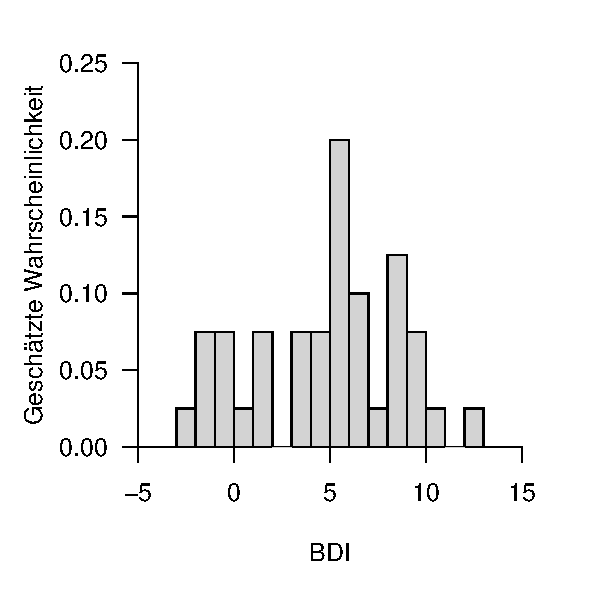
\includegraphics[width=0.45\linewidth]{9_Abbildungen/alm_9_F2F_histogramm} \end{center}

\setstretch{1}
\footnotesize

\begin{Shaded}
\begin{Highlighting}[]
\CommentTok{\# Ausgabe}
\FunctionTok{print.AsIs}\NormalTok{(S)}
\end{Highlighting}
\end{Shaded}

\begin{verbatim}
>      n Max Min Median Mean  Var  Std
> F2F 40  13  -3      6 5.28 14.8 3.85
\end{verbatim}
\end{frame}

\begin{frame}{Einstichproben-T-Tests}
\protect\hypertarget{einstichproben-t-tests-2}{}
\large
\setstretch{3}
\vfill

Anwendungsszenario

\textbf{Modellformulierung}

Modellschätzung

Modellevaluation \vfill
\end{frame}

\begin{frame}{Modellformulierung}
\protect\hypertarget{modellformulierung}{}
\footnotesize
\begin{definition}[Einstichproben-T-Test Modell]
\justifying
$y_i, i = 1,...,n$ seien Zufallsvariablen, die die $n$ Datenpunkte eines Einstichproben-T-Test
Anwendungsszenarios modellieren. Dann hat das \textit{Einstichproben-T-Test Modell}
die strukturelle Form
\begin{equation}
y_i = \mu + \varepsilon_i
\mbox{ mit }
\varepsilon_i \sim N(0,\sigma^2) \mbox{ u.i.v. für } i = 1,...,n \mbox{ mit } \mu \in \mathbb{R} \mbox{ und } \sigma^2 > 0,
\end{equation}
die Datenverteilungsform
\begin{equation}
y_i \sim  N(\mu,\sigma^2) \mbox{ u.i.v. für } i = 1,...,n \mbox{ mit } \mu \in \mathbb{R} \mbox{ und } \sigma^2 > 0,
\end{equation}
und für den Datenvektor $y = (y_1,...,y_n)^T$ die Designmatrixform
\begin{equation}
y = X\beta + \varepsilon \mbox{ mit }
X := 1_n \in \mathbb{R}^{n \times 1},
\beta := \mu \in \mathbb{R},
\varepsilon \sim N(0_n,\sigma^2I_n),
\mbox{ und }
\sigma^2 > 0.
\end{equation}
\end{definition}

Bemerkungen

\begin{itemize}
\tightlist
\item
  Das Modell ist identisch mit dem Modell unabhängiger und identisch
  normalverteilter Zufallsvariablen.
\item
  Es ist \(p = 1\).
\item
  Die Äquivalenz der drei Modellformen wurde in Einheit (5)
  Modellformulierung ausführlich diskutiert.
\end{itemize}
\end{frame}

\begin{frame}[fragile]{Modellformulierung}
\protect\hypertarget{modellformulierung-1}{}
\small

Datensimulation (vgl. Einheit (5) Modellformulierung) \vspace{4mm}

\footnotesize
\setstretch{1.2}

\begin{Shaded}
\begin{Highlighting}[]
\CommentTok{\# Libraries}
\FunctionTok{library}\NormalTok{(MASS)                                }\CommentTok{\# Multivariate Normalverteilung}

\CommentTok{\# Modellformulierung}
\NormalTok{n      }\OtherTok{=} \DecValTok{40}                                  \CommentTok{\# Anzahl von Datenpunkten}
\NormalTok{p      }\OtherTok{=} \DecValTok{1}                                   \CommentTok{\# Anzahl von Betaparameter}
\NormalTok{X      }\OtherTok{=} \FunctionTok{matrix}\NormalTok{(}\FunctionTok{rep}\NormalTok{(}\DecValTok{1}\NormalTok{,n), }\AttributeTok{nrow =}\NormalTok{ n)          }\CommentTok{\# Designmatrix}
\NormalTok{I\_n    }\OtherTok{=} \FunctionTok{diag}\NormalTok{(n)                             }\CommentTok{\# n x n Einheitsmatrix}
\NormalTok{beta   }\OtherTok{=} \DecValTok{5}                                   \CommentTok{\# wahrer, aber unbekannter, Betaparameter}
\NormalTok{sigsqr }\OtherTok{=} \DecValTok{14}                                  \CommentTok{\# wahrer, aber unbekannter, Varianzparameter}

\CommentTok{\# Datenrealisierung}
\NormalTok{y      }\OtherTok{=} \FunctionTok{mvrnorm}\NormalTok{(}\DecValTok{1}\NormalTok{, X }\SpecialCharTok{\%*\%}\NormalTok{ beta, sigsqr}\SpecialCharTok{*}\NormalTok{I\_n)  }\CommentTok{\# eine Realisierung eines n{-}dimensionalen ZVs}
\end{Highlighting}
\end{Shaded}
\end{frame}

\begin{frame}{Einstichproben-T-Tests}
\protect\hypertarget{einstichproben-t-tests-3}{}
\large
\setstretch{3}
\vfill

Anwendungsszenario

Modellformulierung

\textbf{Modellschätzung}

Modellevaluation \vfill
\end{frame}

\begin{frame}{Modellschätzung}
\protect\hypertarget{modellschuxe4tzung}{}
\footnotesize
\begin{theorem}[Parameterschätzung im Einstichproben-T-Test Modell]
\normalfont
\justifying
Gegeben sei die Designmatrixform des Einstichproben-T-Test Modells. Dann ergeben
sich für den Betaparameterschätzer
\begin{equation}
\hat{\beta} = \frac{1}{n}\sum_{i=1}^n y_i =: \bar{y},
\end{equation}
und für den Varianzparameterschätzer
\begin{equation}
\hat{\sigma}^2 = \frac{1}{n-1}\sum_{i=1}^n (y_i - \bar{y})^2 =: s_y^2
\end{equation}
\end{theorem}

Bemerkungen

\begin{itemize}
\tightlist
\item
  Die Formen von \(\hat{\beta}\) und \(\hat{\sigma}^2\) wurden in
  Einheit (6) Modellschätzung hergeleitet.
\item
  \(\bar{y}\) und \(s_y^2\) bezeichnen das Stichprobenmittel und die
  Stichprobenvarianz der \(y_1,...,y_n\).
\end{itemize}
\end{frame}

\begin{frame}[fragile]{Modellschätzung}
\protect\hypertarget{modellschuxe4tzung-1}{}
\tiny
\setstretch{1.2}

\begin{Shaded}
\begin{Highlighting}[]
\CommentTok{\# Dateneinlesen}
\NormalTok{fname       }\OtherTok{=} \FunctionTok{file.path}\NormalTok{(}\FunctionTok{getwd}\NormalTok{(), }\StringTok{"9\_Daten"}\NormalTok{, }\StringTok{"data\_9\_t\_tests.csv"}\NormalTok{)   }\CommentTok{\# Dateiname}
\NormalTok{D           }\OtherTok{=} \FunctionTok{read.table}\NormalTok{(fname, }\AttributeTok{sep =} \StringTok{","}\NormalTok{, }\AttributeTok{header =} \ConstantTok{TRUE}\NormalTok{)           }\CommentTok{\# Dataframe}
\NormalTok{y           }\OtherTok{=}\NormalTok{ D}\SpecialCharTok{$}\NormalTok{BDI[D}\SpecialCharTok{$}\NormalTok{Condition }\SpecialCharTok{==} \StringTok{"F2F"}\NormalTok{]                           }\CommentTok{\# BDI Differenzwerte in der F2F Gruppe}

\CommentTok{\# Modellformulierung}
\NormalTok{n          }\OtherTok{=} \FunctionTok{length}\NormalTok{(y)                                              }\CommentTok{\# Anzahl Datenpunkte}
\NormalTok{p          }\OtherTok{=} \DecValTok{1}                                                      \CommentTok{\# Anzahl Betaparameter}
\NormalTok{X          }\OtherTok{=} \FunctionTok{matrix}\NormalTok{(}\FunctionTok{rep}\NormalTok{(}\DecValTok{1}\NormalTok{,n), }\AttributeTok{nrow =}\NormalTok{ n)                             }\CommentTok{\# Designmatrix}

\CommentTok{\# Modellschätzung}
\NormalTok{beta\_hat   }\OtherTok{=} \FunctionTok{solve}\NormalTok{(}\FunctionTok{t}\NormalTok{(X) }\SpecialCharTok{\%*\%}\NormalTok{ X) }\SpecialCharTok{\%*\%} \FunctionTok{t}\NormalTok{(X) }\SpecialCharTok{\%*\%}\NormalTok{ y                       }\CommentTok{\# Betaparameterschätzer}
\NormalTok{eps\_hat    }\OtherTok{=}\NormalTok{ y }\SpecialCharTok{{-}}\NormalTok{ X }\SpecialCharTok{\%*\%}\NormalTok{ beta\_hat                                     }\CommentTok{\# Residuenvektor}
\NormalTok{sigsqr\_hat }\OtherTok{=}\NormalTok{ (}\FunctionTok{t}\NormalTok{(eps\_hat) }\SpecialCharTok{\%*\%}\NormalTok{ eps\_hat) }\SpecialCharTok{/}\NormalTok{(n}\SpecialCharTok{{-}}\NormalTok{p)                        }\CommentTok{\# Varianzparameterschätzer}

\CommentTok{\# Ausgabe}
\FunctionTok{cat}\NormalTok{(}\StringTok{"hat\{beta\}   : "}\NormalTok{  , beta\_hat,                                   }\CommentTok{\# Betaparameterschätzer}
    \StringTok{"}\SpecialCharTok{\textbackslash{}n}\StringTok{bar\{y\}      : "}\NormalTok{, }\FunctionTok{mean}\NormalTok{(y),                                    }\CommentTok{\# Stichprobenmittel}
    \StringTok{"}\SpecialCharTok{\textbackslash{}n}\StringTok{hat\{sigsqr\} : "}\NormalTok{, sigsqr\_hat,                                 }\CommentTok{\# Varianzparameterschätzer}
    \StringTok{"}\SpecialCharTok{\textbackslash{}n}\StringTok{s\_y\^{}2       : "}\NormalTok{, }\FunctionTok{var}\NormalTok{(y))                                     }\CommentTok{\# Stichprobenvarianz}
\end{Highlighting}
\end{Shaded}

\begin{verbatim}
> hat{beta}   :  5.28 
> bar{y}      :  5.28 
> hat{sigsqr} :  14.8 
> s_y^2       :  14.8
\end{verbatim}
\end{frame}

\begin{frame}{Einstichproben-T-Tests}
\protect\hypertarget{einstichproben-t-tests-4}{}
\large
\setstretch{3}
\vfill

Anwendungsszenario

Modellformulierung

Modellschätzung

\textbf{Modellevaluation} \vfill
\end{frame}

\begin{frame}{Modellevaluation}
\protect\hypertarget{modellevaluation}{}
\setstretch{3}

Überblick

\footnotesize

\begin{itemize}
\tightlist
\item
  Wir gruppieren frequentistische Konfidenzintervalle und
  Hypothesentests unter Modellevaluation.
\item
  Zu Konfidenzintervallen im Szenario u.i.n.v. ZVen siehe WTFI Einheit
  (11) Konfidenzintervalle.
\item
  In der Praxis zielt die Evaluation von Einstichproben-T-Tests ALM
  Designs meist auf einen Hypothesentest.
\item
  Die Theorie des Einstichproben-T-Tests ist umfangreich, siehe dazu
  WTFI (13) Einstichproben T-Tests.
\item
  Wir fokussieren hier auf zweiseitige Einstichproben-T-Tests mit
  ungerichteter Hypothese.
\item
  Ein gutes Verständnis von WTFI Einheit (12) Hypothesentests wird im
  Folgenden vorausgesetzt.
\end{itemize}
\end{frame}

\begin{frame}{Modellevaluation}
\protect\hypertarget{modellevaluation-1}{}
\small

Hypothesenszenarien

\setstretch{1.1}

Einfache Nullhypothese, einfache Alternativhypothese
\(H_0:\mu = \mu_0, H_1:\mu = \mu_1\)

\begin{itemize}
\item Theoretisch wichtiges Szenario (Neymann-Pearson Lemma)
\item Praktische Relevanz eher gering
\end{itemize}

Einfache Nullhypothese, zusammengesetzte Alternativhypothese
\(H_0:\mu = \mu_0, H_1:\mu \neq \mu_0\)

\begin{itemize}
\item Zweiseitiger Einstichproben-T-Test mit ungerichteter Hypothese
\item Ungerichtete Fragestellung nach einem Unterschied
\end{itemize}

Zusammengesetzte Nullhypothese/Alternativhypothese
\(H_0:\mu \le \mu_0, H_1:\mu > \mu_0\)

\begin{itemize}
\item Einseitiger Einstichproben-T-Test mit gerichteter Hypothese
\item Gerichtete Fragestellung nach einem positiven Unterschied
\end{itemize}

Zusammengesetzte Nullhypothese/Alternativhypothese
\(H_0:\mu\ge\mu_0,H_1:\mu<\mu_0\)

\begin{itemize}
\item Gerichtete Fragestellung nach einem negativen Unterschied
\item Qualitativ äquivalente Theorie zum umgekehrten Fall
\end{itemize}
\end{frame}

\begin{frame}{Modellevaluation}
\protect\hypertarget{modellevaluation-2}{}
\small

Hypothesenszenarien

\small

Im Folgenden näher betrachtetes Hypothesenszenario

\setstretch{1.1}

\textcolor{lightgray}{Einfache Nullhypothese, einfache Alternativhypothese $H_0:\mu = \mu_0, H_1:\mu = \mu_1$}

\begin{itemize}
\item[\textcolor{lightgray}{$\bullet$}] \textcolor{lightgray}{Theoretisch wichtiges Szenario (Neymann-Pearson Lemma)}
\item[\textcolor{lightgray}{$\bullet$}] \textcolor{lightgray}{Praktische Relevanz eher gering}
\end{itemize}

Einfache Nullhypothese, zusammengesetzte Alternativhypothese
\(H_0:\mu = \mu_0, H_1:\mu \neq \mu_0\)

\begin{itemize}
\item Zweiseitiger Einstichproben-T-Test mit ungerichteter Hypothese
\item Ungerichtete Fragestellung nach einem Unterschied
\end{itemize}

\textcolor{lightgray}{Zusammengesetzte Nullhypothese/Alternativhypothese $H_0:\mu \le \mu_0, H_1:\mu > \mu_0$}

\begin{itemize}
\item[\textcolor{lightgray}{$\bullet$}] \textcolor{lightgray}{Einseitiger Einstichproben-T-Test mit gerichteter Hypothese}
\item[\textcolor{lightgray}{$\bullet$}] \textcolor{lightgray}{Gerichtete Fragestellung nach einem positiven Unterschied}
\end{itemize}

\textcolor{lightgray}{Zusammengesetzte Nullhypothese/Alternativhypothese $H_0:\mu\ge\mu_0,H_1:\mu<\mu_0$}

\begin{itemize}
\item[\textcolor{lightgray}{$\bullet$}] \textcolor{lightgray}{Gerichtete Fragestellung nach einem negativen Unterschied}
\item[\textcolor{lightgray}{$\bullet$}] \textcolor{lightgray}{Qualitativ äquivalente Theorie zum umgekehrten Fall}
\end{itemize}
\end{frame}

\begin{frame}{Modellevaluation}
\protect\hypertarget{modellevaluation-3}{}
\setstretch{1.8}

\textcolor{darkblue}{Gliederung (vgl. WTFI Einheiten (12) - (14))}

\begin{enumerate}
[(1)]
\item
  Statistisches Modell \checkmark
\item
  Testhypothesen \checkmark
\item
  Teststatistik
\item
  Test
\item
  Analyse der Testgütefunktion
\item
  Testumfangkontrolle
\item
  p-Werte
\item
  Analyse der Powerfunktion
\end{enumerate}
\end{frame}

\begin{frame}{Modellevaluation}
\protect\hypertarget{modellevaluation-4}{}
\noindent (3) Teststatistik

\footnotesize
\begin{theorem}[T-Teststatistik des Einstichproben-T-Tests]
\normalfont
\justifying
Gegeben sei die Designmatrixform des Einstichproben-T-Test Modells. Dann ergibt
sich für die T-Teststatistik mit
\begin{equation}
c := 1 \mbox{ und } c^T\beta_0 =: \mu_0,
\end{equation}
dass
\begin{equation}
T = \sqrt{n}\left(\frac{\bar{y} - \mu_0}{s_y}\right)
\end{equation}
und es gilt
\begin{equation}
T \sim t(\delta, n-1) \mbox{ mit } \delta = \sqrt{n}\left(\frac{\mu - \mu_0}{\sigma}\right)
\end{equation}
\end{theorem}

Bemerkungen

\begin{itemize}
\tightlist
\item
  Das Theorem basiert auf dem T-Teststatistik Theorem in Einheit (7)
  Modellevaluation.
\item
  Die eng verwandte T-Statistik wurde bereits in Einheit (7)
  Modellevaluation hergeleitet.
\end{itemize}
\end{frame}

\begin{frame}{Modellevaluation}
\protect\hypertarget{modellevaluation-5}{}
\noindent (3) Teststatistik

\footnotesize

\underline{Beweis}

Mit dem T-Teststatistik Theorem in Einheit (7) Modellevaluation gilt
\begin{equation}
T
= \frac{c^T \hat{\beta} - c^T \beta_0}{\sqrt{\hat{\sigma}^2 c^T (X^TX)^{-1}c}}
= \frac{1^T \bar{y} - 1^T \mu_0}{\sqrt{s_y^2 1^T (1_n^T1_n)^{-1}1}}
= \sqrt{n}\left(\frac{\bar{y} - \mu_0}{s_y}\right).
\end{equation} \vspace{2mm}

Weiterhin gilt mit demselben Theorem \begin{equation}
\delta
= \frac{c^T \beta - c^T \beta_0}{\sqrt{\sigma^2 c^T (X^TX)^{-1}c}}
= \frac{1^T \mu   - 1^T \mu_0  }{\sqrt{\sigma^2 1^T (1_n^T 1_n)^{-1}1}}
= \sqrt{n}\left(\frac{\mu - \mu_0}{\sigma}\right)
\end{equation}
\end{frame}

\begin{frame}{Modellevaluation}
\protect\hypertarget{modellevaluation-6}{}
\noindent (4) Test

\footnotesize
\begin{definition}[Zweiseitiger Einstichproben-T-Tests]
\justifying
Gegeben sei das Einstichproben-T-Test Modell. Für ein $\mu_0 \in \mathbb{R}$ seien
die einfache Nullhypothese und die zusammengesetzte Alternativhypothese als
\begin{equation}
H_0 : \mu = \mu_0 \Leftrightarrow \Theta_0 := \{\mu_0\}
\mbox{ und }
H_1 : \mu \neq \mu_0 \Leftrightarrow \Theta_1 := \mathbb{R} \setminus \{\mu_0\},
\end{equation}
definiert. Weiterhin sei die T-Teststatistik definiert als
\begin{equation}
T := \sqrt{n}\left(\frac{\bar{y} - \mu_0}{s_y}\right)
\end{equation}
Dann ist der \textit{zweiseitige Einstichproben-T-Tests} definiert als der
kritische Wert-basierten Test
\begin{equation}
\phi(y) := 1_{\{|T| \ge k\}} =
{\begin{cases}
1 & |T| \ge k \\
0 & |T|  <  k
\end{cases}}.
\end{equation}
\end{definition}

Bemerkungen

\begin{itemize}
\tightlist
\item
  Ausführlicher handelt es sich um den \emph{zweiseitigen
  Einstichproben-T-Tests mit ungerichteter Hypothese}.
\end{itemize}
\end{frame}

\begin{frame}{Modellevaluation}
\protect\hypertarget{modellevaluation-7}{}
\noindent (5) Analyse der Testgütefunktion \vspace{1cm}

\small
\begin{theorem}[Testgütefunktion]
\justifying
\normalfont
$\phi$ sei der im obigen Testszenario definierte Test. Dann ist die
Testgütefunktion von $\phi$ gegeben durch
\begin{equation}
q_{\phi} : \mathbb{R} \to [0,1],
\mu \mapsto q_{\phi}(\mu)
:= 1 - \psi(k;d_\mu,n-1) + \psi(-k;d_\mu,n-1)
\end{equation}
wobei $\psi(\cdot; d_\mu, n-1)$  die KVF der nichtzentralen $t$-Verteilung mit
Nichtzentralitätsparameter
\begin{equation}
d_\mu := \sqrt{n}\left(\frac{\mu - \mu_0}{\sigma}\right)
\end{equation}
und Freiheitsgradparameter $n-1$ bezeichnet.
\end{theorem}
\end{frame}

\begin{frame}{Modellevaluation}
\protect\hypertarget{modellevaluation-8}{}
\setstretch{1.1}

\noindent (5) Analyse der Testgütefunktion \vspace{5mm}

\small

\center Testgütefunktion \(q_\phi\) für
\(\sigma^2 = 9, \mu_0 = 4, n = 12\) und \(k = 1,2,3\). \vspace{2mm}
\begin{equation*}
\quad q_{\phi}(\mu) = \mathbb{P}_\mu(\phi = 1)
\end{equation*}

\begin{center}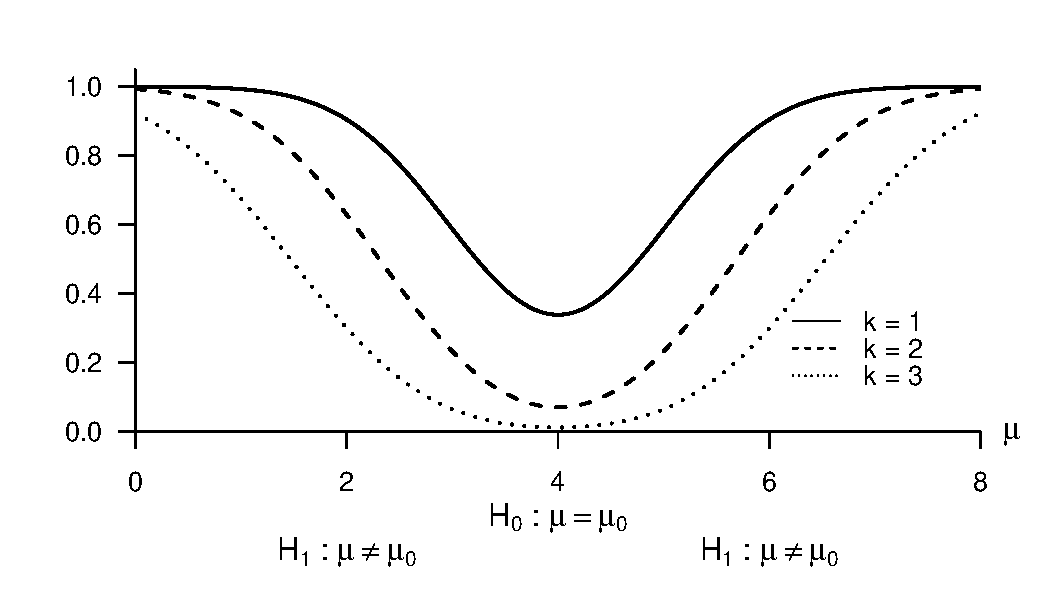
\includegraphics[width=0.8\linewidth]{9_Abbildungen/alm_9_t_test_ungerichtet_guetefunktion} \end{center}
\end{frame}

\begin{frame}{Modellevaluation}
\protect\hypertarget{modellevaluation-9}{}
\setstretch{1.2}

\noindent (5) Analyse der Testgütefunktion

\footnotesize

\underline{Beweis}

Die Testgütefunktion des betrachteten Test im vorliegenden Testszenario
ist definiert als \begin{equation}
q_{\phi} : \mathbb{R} \to [0,1],
\mu \mapsto q_{\phi}(\mu) := \mathbb{P}_{\mu}(\phi = 1).
\end{equation} Da die Wahrscheinlichkeiten für \(\phi = 1\) und dafür,
dass die zugehörige Teststatistik im Ablehnungsbereich des Tests liegt
gleich sind, benötigen wird die also zunächst die Verteilung der
Teststatistik. Wir haben oben bereits gesehen, dass die T-Teststatistik
\begin{equation}
T := \sqrt{n}\left(\frac{\bar{y} - \mu_0}{s_y} \right)
\end{equation} unter der Annahme
\(y_i \sim N(\mu,\sigma^2) \mbox{ u.i.v. für } i = 1,...,n\) nach einer
nichtzentralen \(t\)-Verteilung \(t(d,n-1)\) mit
Nichtzentralitätsparameter \begin{equation}
d = \sqrt{n}\left(\frac{\mu - \mu_0}{\sigma}\right)
\end{equation} verteilt ist. Der Ablehnungsbereich des zweiseitigen
T-Tests ergibt sich, wie in ähnlicher Form bei der Betrachtung des
zweiseitigen Z-Tests gesehen, zu \begin{equation}
A  = \,]-\infty, -k]\, \cup \,]k,\infty[.
\end{equation} \vfill
\end{frame}

\begin{frame}{Modellevaluation}
\protect\hypertarget{modellevaluation-10}{}
\setstretch{1.2}

\noindent (5) Analyse der Testgütefunktion

\footnotesize

\underline{Beweis (fortgeführt)}

Mit diesem Ablehungsbereich ergibt sich dann \begin{align}
\begin{split}
q_\phi(\mu)
& = \mathbb{P}_{\mu}(\phi = 1)                                                   \\
& = \mathbb{P}_{\mu}\left(T \in ]-\infty, -k]\,
                         \cup \,]k,\infty[ \right)                               \\
& = \mathbb{P}_{\mu}\left(T \in ]-\infty, -k]\right)
  + \mathbb{P}_{\mu}\left(T \in [k,\infty[ \right)                               \\
& = \mathbb{P}_{\mu}(T \le -k)  + \mathbb{P}_{\mu}(T \ge k)                      \\
& = \mathbb{P}_{\mu}(T \le -k)  + (1-\mathbb{P}_{\mu}(T \le k))                  \\
& = 1 - \mathbb{P}_{\mu}(T \le k)  + \mathbb{P}_{\mu}(T \le - k)                 \\
& = 1 - \psi(k; d_\mu, n-1)  + \psi(-k;d_\mu,n-1),
\end{split}
\end{align} wobei \(\psi(\cdot; d_\mu,n-1)\) die KVF der nichtzentralen
T-Verteilung mit Nichtzentralitätsparameter \(d_\mu\) und
Freiheitsgradparameter \(n-1\) bezeichnet.

\(\hfill\Box\) \vfill
\end{frame}

\begin{frame}{Modellevaluation}
\protect\hypertarget{modellevaluation-11}{}
\setstretch{1.2}

\noindent (6) Testumfangkontrolle \vfill \small

\begin{theorem}[Testumfangkontrolle]
\justifying
\normalfont
$\phi$ sei der im obigen Testszenario definierte Test. Dann ist $\phi$ ein
Level-$\alpha_0$-Test mit Testumfang $\alpha_0$, wenn der kritische Wert
definiert ist durch
\begin{equation}
k_{\alpha_0} := \psi^{-1}\left(1 - \frac{\alpha_0}{2}; n-1 \right),
\end{equation}
wobei $\psi^{-1}(\cdot; n-1)$ die inverse KVF der $t$-Verteilung mit $n-1$
Freiheitsgraden ist.
\end{theorem}
\vfill
\end{frame}

\begin{frame}{Modellevaluation}
\protect\hypertarget{modellevaluation-12}{}
\setstretch{1.1}

\noindent (6) Testumfangkontrolle \setstretch{1.2}

\footnotesize

\underline{Beweis}

Damit der betrachtete Test ein Level-\(\alpha_0\)-Test ist, muss
bekanntlich \(q_\phi(\mu) \le \alpha_0\) für alle \(\mu \in \{\mu_0\}\),
also hier \(q_\phi(\mu_0) \le \alpha_0\), gelten. Weiterhin ist der
Testumfang des betrachteten Tests durch
\(\alpha = \max_{\mu \in \{\mu_0\}} q_\phi(\mu)\), also hier durch
\(\alpha = q_\phi(\mu_0)\) gegeben. Wir müssen also zeigen, dass die
Wahl von \(k_{\alpha_0}\) garantiert, dass \(\phi\) ein
Level-\(\alpha_0\)-Test mit Testumfang \(\alpha_0\) ist. Dazu merken wir
zunächst an, dass für \(\mu = \mu_0\) gilt, dass \begin{align}
\begin{split}
q_\phi(\mu_0)
& =  1 - \psi(k;d_{\mu_0},n-1) + \psi(-k;d_{\mu_0},n-1)                          \\
& =  1 - \psi(k;0,n-1) + \psi(-k;0,n-1)                                          \\
& =  1 - \psi(k;n-1) + \psi(-k;n-1),                                             \\
\end{split}
\end{align} wobei \(\psi(\cdot;d,n-1)\) und \(\psi(\cdot;n-1)\) die KVF
der nichtzentralen \(t\)-Verteilung mit Nichtzentralitätsparameter \(d\)
und Freiheitsgradparameter \(n-1\) sowie der \(t\)-Verteilung mit
Freiheitsgradparameter \(n-1\), respektive, bezeichnen. Sei nun also
\(k := k_{\alpha_0}\). Dann gilt \begin{align}
\begin{split}
q_\phi(\mu_0)
& = 1 - \psi(k_{\alpha_0}, n-1) + \psi(-k_{\alpha_0}, n-1)                                 \\
& = 1 - \psi(k_{\alpha_0}, n-1) + (1 - \psi(k_{\alpha_0}), n-1)                            \\
& = 2(1-\psi(k_{\alpha_0}, n-1))                                                      \\
& = 2\left(1-\psi\left(\psi^{-1}\left(1 - \alpha_0/2 , n-1\right), n-1\right)\right) \\
& = 2\left(1 - 1 + \alpha_0/2\right)                          \\
& = \alpha_0,
\end{split}
\end{align} wobei die zweite Gleichung mit der Symmetrie der
\(t\)-Verteilung folgt. Es folgt also direkt, dass bei der Wahl von
\(k = k_{\alpha_0}\), \(q_\phi(\mu_0)\le \alpha_0\) ist und der
betrachtete Test somit ein Level-\(\alpha_0\)-Test ist. Weiterhin folgt
direkt, dass der Testumfang des betrachteten Tests bei der Wahl von
\(k = k_{\alpha_0}\) gleich \(\alpha_0\) ist.
\end{frame}

\begin{frame}{Modellevaluation}
\protect\hypertarget{modellevaluation-13}{}
\setstretch{1.2}

\noindent (6) Testumfangkontrolle \small \vfill \center Wahl von
\(k_{\alpha_0} := \psi^{-1}(1 - \alpha_0/2; n-1)\) mit \(n =12\),
\(\alpha_0 := 0.05\) und Ablehnungsbereich \vspace{3mm}

\begin{center}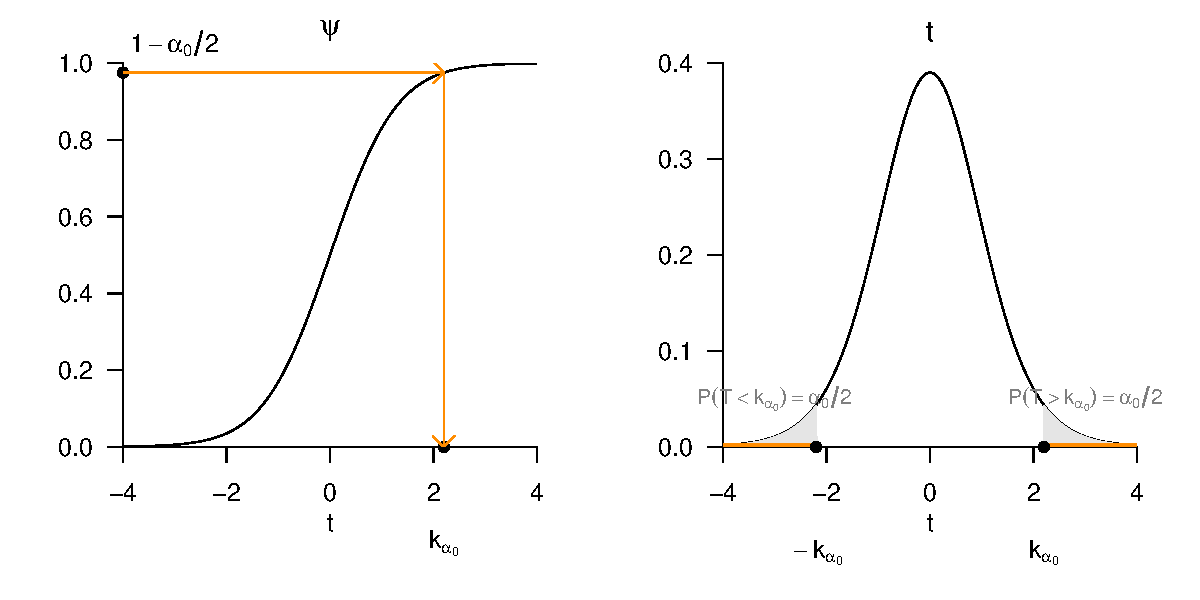
\includegraphics[width=0.8\linewidth]{9_Abbildungen/alm_9_t_test_ungerichtet_testumfangkontrolle} \end{center}
\end{frame}

\begin{frame}{Modellevaluation}
\protect\hypertarget{modellevaluation-14}{}
\justifying
\setstretch{1.2}

\noindent (6) Testumfangkontrolle \vspace{1mm}

Praktisches Vorgehen \small

\begin{itemize}
\item
  \justifying Man nimmt an, dass ein Datensatz
  \(\upsilon_1,...,\upsilon_n\) eine Realisation von
  \(y_i \sim N(\mu,\sigma^2) \mbox{ u.i.v. für } i = 1,...,n\) mit
  unbekannten Parametern \(\mu\) und \(\sigma^2 > 0\) ist.
\item
  Man möchte entscheiden ob für ein \(\mu_0 \in \mathbb{R}\) eher
  \(H_0 : \mu = \mu_0\) oder \(H_1: \mu \neq \mu_0\) zutrifft.

  \item

  Man wählt ein Signifikanzniveau \(\alpha_0\) und bestimmt den
  zugehörigen Freiheitsgradparameter-abhängigen kritischen Wert
  \(k_{\alpha_0}\). Zum Beispiel gilt bei Wahl von \(\alpha_0 := 0.05\)
  und \(n=12\), also Freiheitsgradparameter 11, dass
  \(k_{0.05}=\psi^{-1}(1 - 0.05/2; 11) \approx 2.20\) ist.
\item
  Anhand von \(n, \mu_0, \bar{\upsilon}\) und \(s_\upsilon\) berechnet
  man die Realisierung der T-Teststatistik \begin{equation}
  t := \sqrt{n}\left(\frac{\bar{\upsilon} - \mu_0}{s_\upsilon}\right)
  \end{equation}
\item
  Wenn \(t\) größer-gleich \(k_{\alpha_0}\) ist oder wenn \(t\) kleiner-
  gleich \(-k_{\alpha_0}\) ist, lehnt man die Nullhypothese ab,
  andernfalls lehnt man sie nicht ab.
\item
  Die oben entwickelte Theorie garantiert dann, dass man in höchstens
  \(\alpha_0 \cdot 100\) von \(100\) Fällen die Nullhypothese
  fälschlicherweise ablehnt.
\end{itemize}
\end{frame}

\begin{frame}{Modellevaluation}
\protect\hypertarget{modellevaluation-15}{}
\noindent (7) p-Werte

\small

Bestimmung des p-Wertes \vspace{2mm}

\begin{itemize}
\item
  \itemsep2mm \justifying Per Definition ist der p-Wert das kleinste
  Signifikanzlevel \(\alpha_0\), bei welchem man die Nullhypothese
  basierend auf einem vorliegendem Wert der Teststatistik ablehnen
  würde.
\item
  Bei \(T = t\) würde \(H_0\) für jedes \(\alpha_0\) mit
  \(|t| \ge \psi^{-1}(1-\alpha_0/2; n-1)\) abgelehnt werden. Für diese
  \(\alpha_0\) gilt, wie unten gezeigt, \begin{equation}
  \alpha_0 \ge 2 \mathbb{P}(T \ge |t|).
  \end{equation}
\item
  Das kleinste \(\alpha_0 \in [0,1]\) mit
  \(\alpha_0 \ge 2 \mathbb{P}(T \ge |t|)\) ist dann
  \(\alpha_0 = 2 \mathbb{P}(T \ge |t|)\), also folgt \begin{equation}
  \mbox{p-Wert} =  2 \mathbb{P}(T \ge |t|) = 2(1 - \psi(|t|;n-1)).
  \end{equation}
\item
  Im Gegensatz zum Z-Test hängt bei T-Tests der p-Wert auch von der
  Stichprobengröße ab.
\item
  Zum Beispiel ist für \(T = 2.00\) und \(n = 10\) der p-Wert \(0.076\),
  für \(T = 2.00\) und \(n = 100\) ist der p-Wert dagegen \(0.048\).
\end{itemize}
\end{frame}

\begin{frame}{Modellevaluation}
\protect\hypertarget{modellevaluation-16}{}
\noindent (7) p-Werte

\small

Bestimmung des p-Wertes \vspace{2mm}

\begin{itemize}
\item
  \itemsep2mm \justifying Es bleibt zu zeigen, dass gilt
  \begin{equation}
  |t| \ge \psi^{-1}(1 - \alpha_0/2; n-1)
  \Leftrightarrow
  \alpha_0 \ge 2 \mathbb{P}(T \ge |t|)
  \end{equation}
\item
  Dies aber folgt aus \footnotesize \vspace{-2mm} \begin{align}
  \begin{split}
  |t|
  & \ge \psi^{-1}\left(1 - \frac{\alpha_0}{2}; n-1\right)
  \\\Leftrightarrow
  \psi(|t|; n-1)
  & \ge \psi\left(\psi^{-1}\left(1 - \frac{\alpha_0}{2}; n-1\right); n-1\right)
  \\\Leftrightarrow
  \psi(|t|; n-1)
  & \ge 1 - \frac{\alpha_0}{2}
  \\\Leftrightarrow
  \mathbb{P}(T \le |t|)
  & \ge 1 - \frac{\alpha_0}{2}
  \\\Leftrightarrow
  \frac{\alpha_0}{2}
  & \ge 1 - \mathbb{P}(T \le |t|)
  \\\Leftrightarrow
  \frac{\alpha_0}{2}
  & \ge \mathbb{P}(T \ge |t|)
  \\\Leftrightarrow
  \alpha_0
  & \ge 2 \mathbb{P}(T \ge |t|).
  \end{split}
  \end{align}
\end{itemize}
\end{frame}

\begin{frame}[fragile]{Modellevaluation}
\protect\hypertarget{modellevaluation-17}{}
\vspace{1mm}
\small

\textcolor{darkblue}{Anwendungszenario} \vspace{1mm} \setstretch{.9}
\tiny

\begin{Shaded}
\begin{Highlighting}[]
\CommentTok{\# Dateneinlesen}
\NormalTok{fname       }\OtherTok{=} \FunctionTok{file.path}\NormalTok{(}\FunctionTok{getwd}\NormalTok{(), }\StringTok{"9\_Daten"}\NormalTok{, }\StringTok{"data\_9\_t\_tests.csv"}\NormalTok{)  }\CommentTok{\# Dateiname}
\NormalTok{D           }\OtherTok{=} \FunctionTok{read.table}\NormalTok{(fname, }\AttributeTok{sep =} \StringTok{","}\NormalTok{, }\AttributeTok{header =} \ConstantTok{TRUE}\NormalTok{)          }\CommentTok{\# Dataframe}
\NormalTok{y           }\OtherTok{=}\NormalTok{ D}\SpecialCharTok{$}\NormalTok{BDI[D}\SpecialCharTok{$}\NormalTok{Condition }\SpecialCharTok{==} \StringTok{"F2F"}\NormalTok{]                          }\CommentTok{\# BDI Differenzwerte in der F2F Gruppe}

\CommentTok{\# Modellformulierung}
\NormalTok{n          }\OtherTok{=} \FunctionTok{length}\NormalTok{(y)                                             }\CommentTok{\# Anzahl Datenpunkte}
\NormalTok{p          }\OtherTok{=} \DecValTok{1}                                                     \CommentTok{\# Anzahl Betaparameter}
\NormalTok{X          }\OtherTok{=} \FunctionTok{matrix}\NormalTok{(}\FunctionTok{rep}\NormalTok{(}\DecValTok{1}\NormalTok{,n), }\AttributeTok{nrow =}\NormalTok{ n)                            }\CommentTok{\# Designmatrix}

\CommentTok{\# Modellschätzung}
\NormalTok{beta\_hat   }\OtherTok{=} \FunctionTok{solve}\NormalTok{(}\FunctionTok{t}\NormalTok{(X) }\SpecialCharTok{\%*\%}\NormalTok{ X) }\SpecialCharTok{\%*\%} \FunctionTok{t}\NormalTok{(X) }\SpecialCharTok{\%*\%}\NormalTok{ y                      }\CommentTok{\# Betaparameterschätzer}
\NormalTok{eps\_hat    }\OtherTok{=}\NormalTok{ y }\SpecialCharTok{{-}}\NormalTok{ X }\SpecialCharTok{\%*\%}\NormalTok{ beta\_hat                                    }\CommentTok{\# Residuenvektor}
\NormalTok{sigsqr\_hat }\OtherTok{=}\NormalTok{ (}\FunctionTok{t}\NormalTok{(eps\_hat) }\SpecialCharTok{\%*\%}\NormalTok{ eps\_hat) }\SpecialCharTok{/}\NormalTok{(n}\SpecialCharTok{{-}}\NormalTok{p)                       }\CommentTok{\# Varianzparameterschätzer}

\CommentTok{\# Modellevaluation}
\NormalTok{c          }\OtherTok{=} \FunctionTok{matrix}\NormalTok{(}\FunctionTok{c}\NormalTok{(}\DecValTok{1}\NormalTok{),}\AttributeTok{nrow =}\NormalTok{ p)                                 }\CommentTok{\# Kontrastgewichtsvektor}
\NormalTok{mu\_0       }\OtherTok{=} \DecValTok{0}                                                     \CommentTok{\# Nullhypothese H\_0}
\NormalTok{alpha\_0    }\OtherTok{=} \FloatTok{0.05}                                                  \CommentTok{\# Signifikanzniveau}
\NormalTok{k\_alpha\_0  }\OtherTok{=} \FunctionTok{qt}\NormalTok{(}\DecValTok{1} \SpecialCharTok{{-}}\NormalTok{ (alpha\_0}\SpecialCharTok{/}\DecValTok{2}\NormalTok{), n}\DecValTok{{-}1}\NormalTok{)                              }\CommentTok{\# kritischer Wert}
\NormalTok{t\_num      }\OtherTok{=} \FunctionTok{t}\NormalTok{(c) }\SpecialCharTok{\%*\%}\NormalTok{ beta\_hat }\SpecialCharTok{{-}}\NormalTok{ mu\_0                              }\CommentTok{\# T{-}Teststatistik Zähler}
\NormalTok{t\_den      }\OtherTok{=} \FunctionTok{sqrt}\NormalTok{(sigsqr\_hat }\SpecialCharTok{\%*\%} \FunctionTok{t}\NormalTok{(c)}\SpecialCharTok{*}\FunctionTok{solve}\NormalTok{(}\FunctionTok{t}\NormalTok{(X) }\SpecialCharTok{\%*\%}\NormalTok{ X)}\SpecialCharTok{\%*\%}\NormalTok{c)       }\CommentTok{\# T{-}Teststatistik Nenner}
\NormalTok{t          }\OtherTok{=}\NormalTok{ t\_num}\SpecialCharTok{/}\NormalTok{t\_den                                           }\CommentTok{\# T{-}Teststatistik}
\ControlFlowTok{if}\NormalTok{(}\FunctionTok{abs}\NormalTok{(t) }\SpecialCharTok{\textgreater{}=}\NormalTok{ k\_alpha\_0)\{                                           }\CommentTok{\# Test 1\_\{|T(X) \textgreater{}= k\_alpha\_0|\}}
\NormalTok{    phi }\OtherTok{=} \DecValTok{1}                                                        \CommentTok{\# Ablehnen von H\_0}
\NormalTok{\} }\ControlFlowTok{else}\NormalTok{ \{}
\NormalTok{    phi }\OtherTok{=} \DecValTok{0}                                                        \CommentTok{\# Nicht Ablehnen von H\_0}
\NormalTok{\}}
\NormalTok{pval      }\OtherTok{=} \DecValTok{2}\SpecialCharTok{*}\NormalTok{(}\DecValTok{1} \SpecialCharTok{{-}} \FunctionTok{pt}\NormalTok{(}\FunctionTok{abs}\NormalTok{(t), n}\DecValTok{{-}1}\NormalTok{))                                }\CommentTok{\# p{-}Wert}
\end{Highlighting}
\end{Shaded}

\vspace{-2mm}

\begin{verbatim}
> fg        =  39 
> t         =  8.67 
> alpha_0   =  0.05 
> k_alpha_0 =  2.02 
> phi       =  1 
> p-Wert    =  1.25e-10
\end{verbatim}
\end{frame}

\begin{frame}[fragile]{Modellevaluation}
\protect\hypertarget{modellevaluation-18}{}
\small

\textcolor{darkblue}{Anwendungszenario} \vspace{2mm}

\setstretch{1.1}
\tiny

\begin{Shaded}
\begin{Highlighting}[]
\CommentTok{\# Automatischer Einstichproben{-}T{-}Test}
\NormalTok{varphi    }\OtherTok{=} \FunctionTok{t.test}\NormalTok{(                           }\CommentTok{\# ?t.test für Details}
\NormalTok{            y,                                }\CommentTok{\# Datensatz}
            \AttributeTok{alternative =} \FunctionTok{c}\NormalTok{(}\StringTok{"two.sided"}\NormalTok{),     }\CommentTok{\# H\_1: \textbackslash{}mu \textbackslash{}neq \textbackslash{}mu\_0}
            \AttributeTok{mu          =} \DecValTok{0}\NormalTok{,                  }\CommentTok{\# \textbackslash{}mu\_0 (sic!)}
            \AttributeTok{conf.level  =} \DecValTok{1}\SpecialCharTok{{-}}\NormalTok{alpha\_0)          }\CommentTok{\# \textbackslash{}delta = 1 {-} \textbackslash{}alpha\_0 (sic!)}

\CommentTok{\# Ausgabe}
\FunctionTok{print}\NormalTok{(varphi)}
\end{Highlighting}
\end{Shaded}

\begin{verbatim}
> 
>   One Sample t-test
> 
> data:  y
> t = 9, df = 39, p-value = 1e-10
> alternative hypothesis: true mean is not equal to 0
> 95 percent confidence interval:
>  4.04 6.51
> sample estimates:
> mean of x 
>      5.28
\end{verbatim}

\begin{Shaded}
\begin{Highlighting}[]
\CommentTok{\# Genauere Ausgabe t}
\FunctionTok{paste}\NormalTok{(varphi[}\DecValTok{1}\NormalTok{])}
\end{Highlighting}
\end{Shaded}

\begin{verbatim}
> [1] "c(t = 8.66623050649246)"
\end{verbatim}

\begin{Shaded}
\begin{Highlighting}[]
\CommentTok{\# Genauere Ausgabe p}
\FunctionTok{paste}\NormalTok{(varphi[}\DecValTok{3}\NormalTok{])}
\end{Highlighting}
\end{Shaded}

\begin{verbatim}
> [1] "1.25177126014618e-10"
\end{verbatim}
\end{frame}

\begin{frame}{Modellevaluation}
\protect\hypertarget{modellevaluation-19}{}
\noindent (8) Analyse der Powerfunktion \vfill \justifying

\small

Wir betrachten die Testgütefunktion \begin{equation}
q_\phi : \mathbb{R} \to [0,1],
\mu \mapsto q_\phi(\mu)
:= 1 - \psi(k_{\alpha_0}; d_\mu, n-1) + \psi(-k_{\alpha_0}; d_\mu, n-1)
\end{equation} bei kontrolliertem Testumfang, also für
\(k_{\alpha_0} := \psi^{-1}(1-\alpha_0/2;n-1)\) mit festem \(\alpha_0\)
als Funktion des Nichtzentralitätsparameters und des Stichprobenumfangs.
Namentlich hängt hier \(k_{\alpha_0}\) auch von \(n\) ab.

Es ergibt sich die bivariate reellwertige Funktion \begin{equation}
\pi : \mathbb{R} \times \mathbb{N} \to [0,1],
(d,n) \mapsto
\pi(d,n) := 1 - \psi(k_{\alpha_0}; d, n-1) + \psi(-k_{\alpha_0}; d, n-1)
\end{equation} Bei festgelegten \(\alpha_0\) hängt die Powerfunktion des
zweiseitigen T-Tests mit einfacher Nullhypothese also vom unbekannten
Wert \(d\) und von der Stichprobengröße \(n\) ab. Wir visualisieren
diese Abhängigkeiten untenstehend. \vfill
\end{frame}

\begin{frame}{Modellevaluation}
\protect\hypertarget{modellevaluation-20}{}
\begin{enumerate}
[(1)]
\setcounter{enumi}{7}
\tightlist
\item
  Analyse der Powerfunktion
\end{enumerate}

\small

Powerfunktion für \(\alpha_0 = 0.05\)

\begin{center}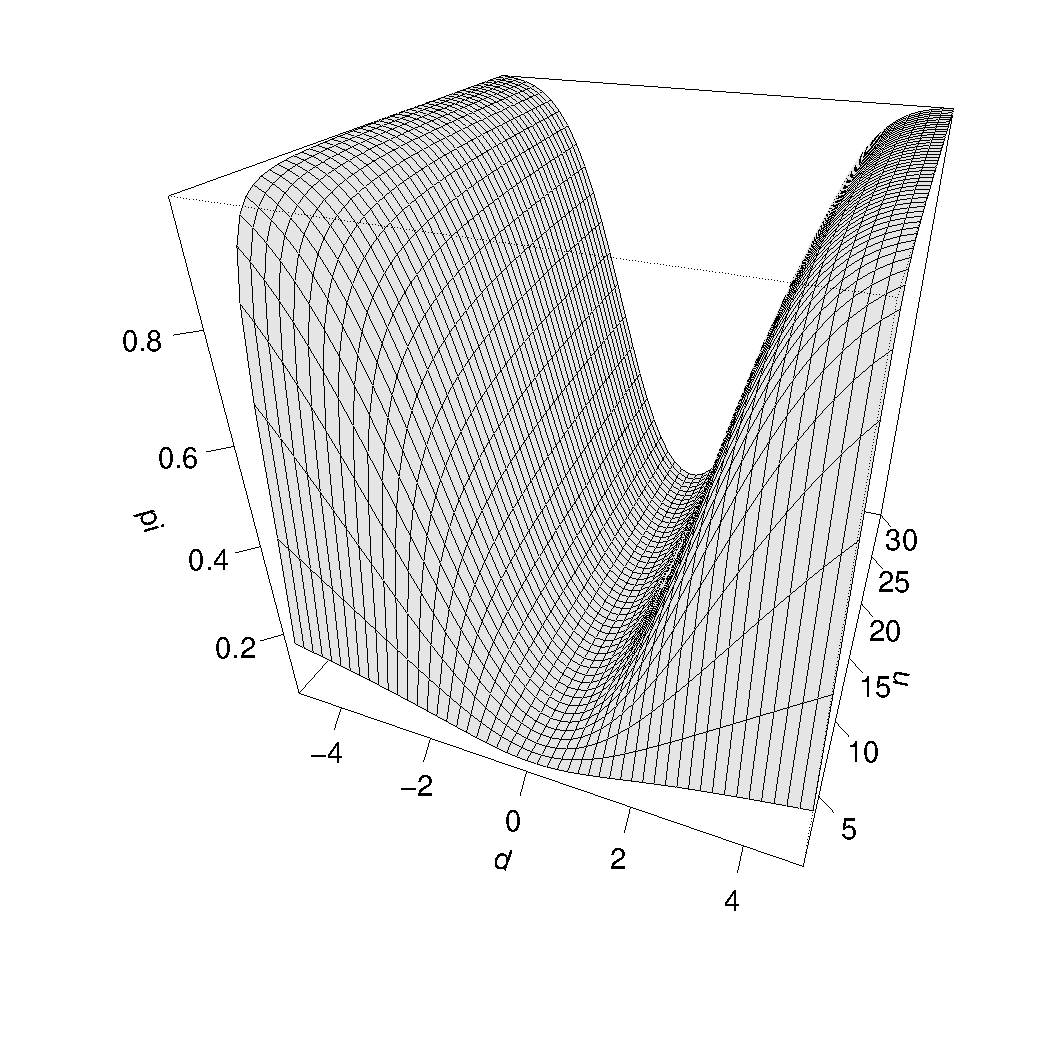
\includegraphics[width=0.6\linewidth]{9_Abbildungen/alm_9_t_test_ungerichtet_power_005} \end{center}
\end{frame}

\begin{frame}{Zweiseitige Einstichproben-T-Tests}
\protect\hypertarget{zweiseitige-einstichproben-t-tests}{}
\begin{enumerate}
[(1)]
\setcounter{enumi}{7}
\tightlist
\item
  Analyse der Powerfunktion
\end{enumerate}

\small

Powerfunktion für \(\alpha_0 = 0.001\)

\begin{center}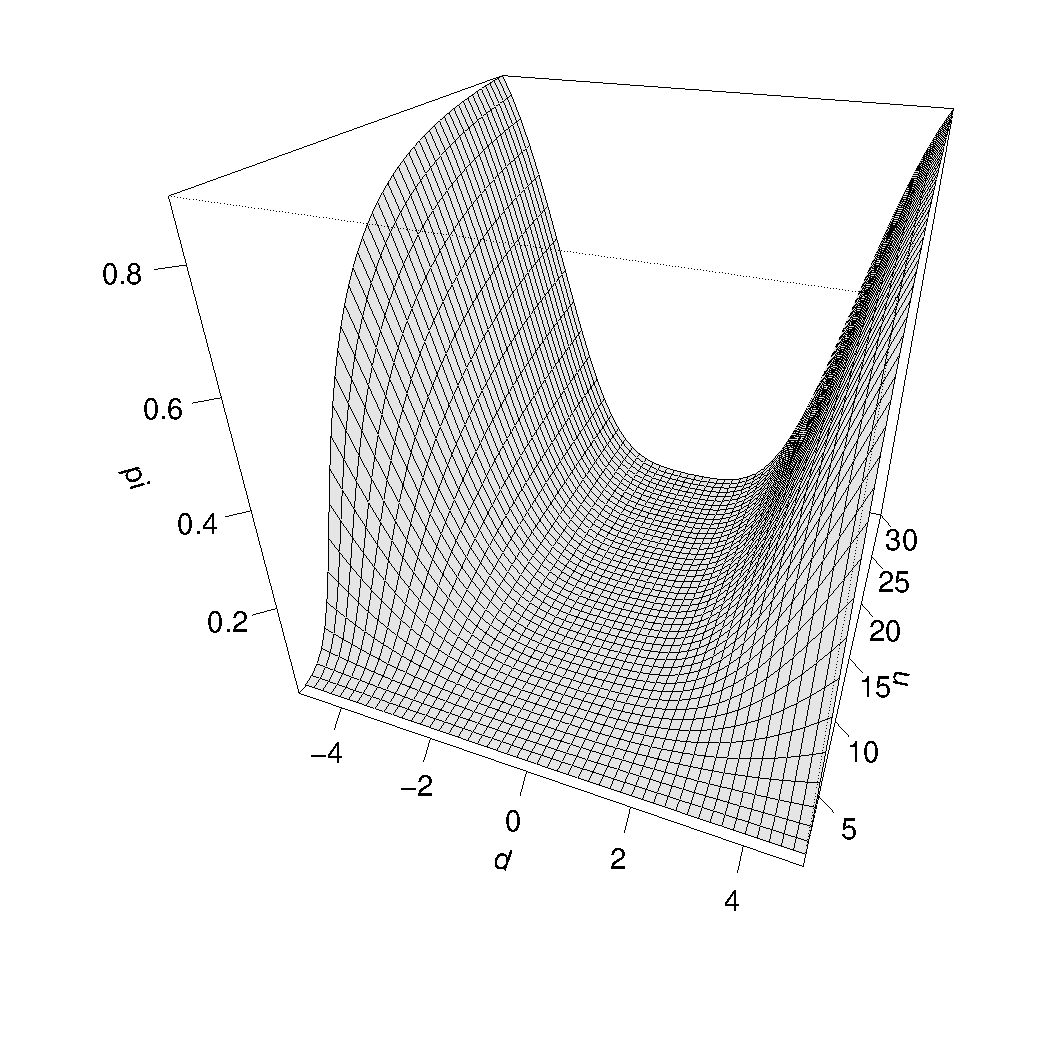
\includegraphics[width=0.6\linewidth]{9_Abbildungen/alm_9_t_test_ungerichtet_power_0001} \end{center}
\end{frame}

\begin{frame}{Modellevaluation}
\protect\hypertarget{modellevaluation-21}{}
\begin{enumerate}
[(1)]
\setcounter{enumi}{7}
\tightlist
\item
  Analyse der Powerfunktion
\end{enumerate}

\small
\justifying

Powerfunktionen für \(\mu_0 = 0\) \vspace{2mm}

\begin{center}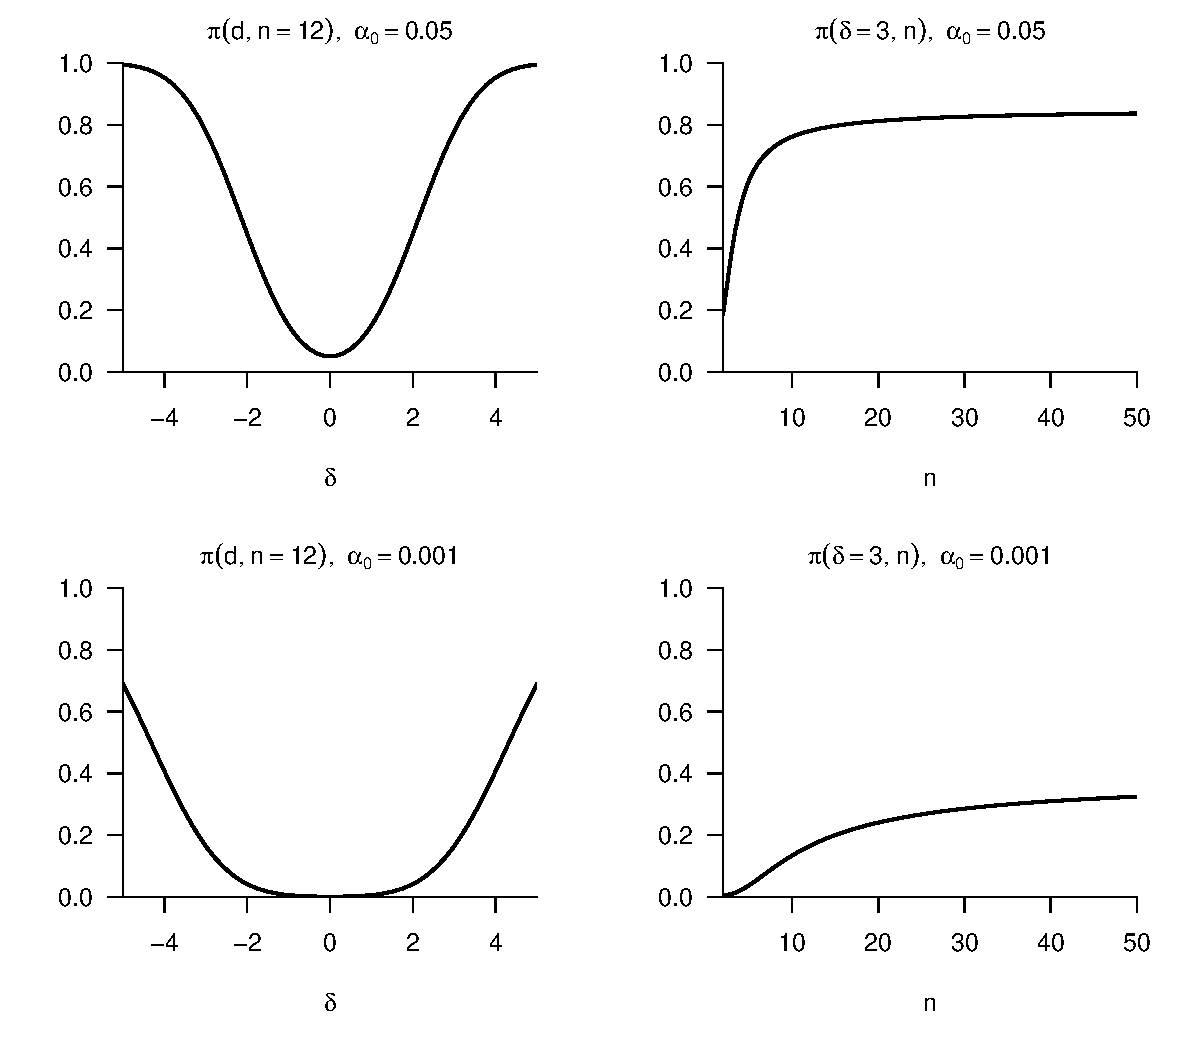
\includegraphics[width=0.65\linewidth]{9_Abbildungen/alm_9_t_test_ungerichtet_powerfunktionen} \end{center}
\end{frame}

\begin{frame}{Modellevaluation}
\protect\hypertarget{modellevaluation-22}{}
\noindent (8) Analyse der Powerfunktion

Praktisches Vorgehen \small

Mit größerem \(n\) steigt die Powerfunktion des Tests an

\begin{itemize}
\item
  Ein großer Stichprobenumfang ist besser als ein kleiner
  Stichprobenumfang.
\item
  Kosten für die Erhöhung des Stichprobenumfangs werden aber nicht
  berücksichtigt.
\end{itemize}

\(\Rightarrow\) Die Theorie statistischer Hypothesentests ist nicht
besonders lebensnah.

\vspace{1mm}

Die Powerfunktion hängt vom wahren, aber unbekannten, Parameterwert
\(d = \sqrt{n}(\mu - \mu_0)/\sigma\) ab.

\(\Rightarrow\) Wenn man \(d\) schon kennen würde, würde man den Test
nicht durchführen.

\vspace{1mm}

Generell wird folgendes Vorgehen favorisiert

\begin{itemize}
\item
  Man legt das Signifikanzniveau \(\alpha_0\) fest und evaluiert die
  Powerfunktion.
\item
  Man wählt einen Mindestparameterwert \(d^*\), den man mit
  \(\pi(d,n) = b\) detektieren möchte.
\item
  Ein konventioneller Wert ist \(b = 0.8\).
\item
  Man liest die für \(\pi(d = d^*,n) = b\) nötige Stichprobengröße \(n\)
  ab.
\end{itemize}
\end{frame}

\begin{frame}{Modellevaluation}
\protect\hypertarget{modellevaluation-23}{}
\noindent (8) Analyse der Powerfunktion

Praktisches Vorgehen \vspace{5mm}

\begin{center}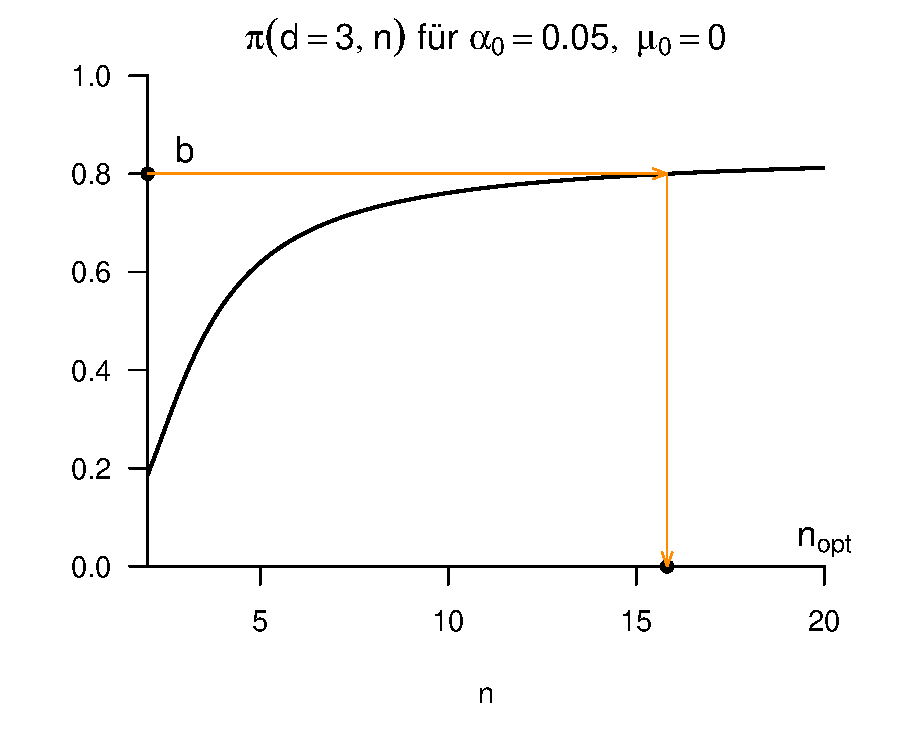
\includegraphics[width=0.6\linewidth]{9_Abbildungen/alm_9_t_test_ungerichtet_stichprobengroesse} \end{center}
\end{frame}

\begin{frame}[plain]{}
\protect\hypertarget{section-6}{}
\large
\setstretch{3}
\vfill

Überblick

Einstichproben-T-Tests

\textbf{Zweistichproben-T-Tests}

Selbstkontrollfragen \vfill
\end{frame}

\begin{frame}[plain]{}
\protect\hypertarget{section-7}{}
\center
\huge
\vfill

\noindent Zweistichproben-T-Tests \vfill
\end{frame}

\begin{frame}{Zweistichproben-T-Tests}
\protect\hypertarget{zweistichproben-t-tests}{}
\large
\setstretch{3}
\vfill

Anwendungsszenario

Modellformulierung

Modellschätzung

Modellevaluation \vfill
\end{frame}

\begin{frame}{Zweistichproben-T-Tests}
\protect\hypertarget{zweistichproben-t-tests-1}{}
\large
\setstretch{3}
\vfill

\textbf{Anwendungsszenario}

Modellformulierung

Modellschätzung

Modellevaluation \vfill
\end{frame}

\begin{frame}{Anwendungsszenario}
\protect\hypertarget{anwendungsszenario-6}{}
\textbf{\textcolor{darkblue}{Zwei Gruppen}} (Stichproben) randomisierter
experimenteller Einheiten.

Annahme unabhängiger identischer Normalverteilungen
\(N(\mu_1,\sigma^2)\) und \(N(\mu_2,\sigma^2)\).

\(\mu_1,\mu_2\) und \(\sigma^2\) unbekannt.

Annahme eines identischen Varianzparameters für beide Gruppen.

Quantifizieren der Unsicherheit beim inferentiellen Vergleich von
\(\mu_1\) mit \(\mu_2\) beabsichtigt.

\vspace{2mm}

\textcolor{darkblue}{Anwendungsbeispiele}

\small

BDI Differenzwert Datenanalyse bei zwei Gruppen von Patient:innen
\vspace{-2mm}

\begin{itemize}
\tightlist
\item
  Gruppe 1 Face-to-Face Therapie, Gruppe 2 Online Therapie
\item
  \(\mu_1 \neq \mu_2 \Leftrightarrow\) Unterscheiden sich die
  Therapiewirksamkeiten?
\end{itemize}

Forcierte Schwimmtestdatenanalyse bei zwei Gruppen genmanipulierter
Mäuse \vspace{-2mm}

\begin{itemize}
\tightlist
\item
  Gruppe 1 Wildtyp, Gruppe 2 Serotoninrezeptormutation
\item
  \(\mu_1 \neq \mu_2 \Leftrightarrow\) Trägt Serotoninrezeptor zum
  Schwimmtestverhalten bei?
\end{itemize}
\end{frame}

\begin{frame}{Anwendungsszenario}
\protect\hypertarget{anwendungsszenario-7}{}
\small

Wir betrachten das Anwendungsbeispiel aus Einheit (8) Studiendesign und
fokussieren auf die Gruppen (= Stichproben, Experimentalbedingungen) der
Face-to-Face und der Online Therapie. Wir betrachten dabei wieder den
Datensatz der negativen PostBDI-PreBDI Differenzwerte mit Variablennamen
``BDI.'' \vspace{3mm}

Wir nehmen an, dass die Datenpunkte der Face-to-Face Therapiegruppe
u.i.v. Realisierungen von ZVen \(y_{1j} \sim N(\mu_1,\sigma^2)\) für
\(j = 1,...,40\) und dass die Datenpunkte der Online Therapiegruppe
u.i.v. Realisierungen von ZVen \(y_{2j} \sim N(\mu_2,\sigma^2)\) für
\(j = 1,...,40\) sind. Wir nehmen weiter an, dass wir an der
Quantifizierung der Unsicherheit beim inferentiellen Vergleich der
wahren, aber unbekannt, Erwartungswertparameter \(\mu_1\) und \(\mu_2\)
im Sinne eines Hypothesentests interessiert sind. \vspace{3mm}

Im Folgenden evaluieren den hier betrachteten Datensatz zunächst im
Sinne deskriptiver Statistiken, siehe dazu auch Einheit (11)
Anwendungsbeispiel in Programmierung und Deskriptive Statistik.
\end{frame}

\begin{frame}[fragile]{Anwendungsszenario}
\protect\hypertarget{anwendungsszenario-8}{}
\vspace{3mm}
\small

\textcolor{darkblue}{Dateneinlesen $\vert$ $j = 1,...,20$ für jede Gruppe}
\setstretch{.6} \tiny \vspace{1mm}

\begin{Shaded}
\begin{Highlighting}[]
\NormalTok{fname       }\OtherTok{=} \FunctionTok{file.path}\NormalTok{(}\FunctionTok{getwd}\NormalTok{(), }\StringTok{"9\_Daten"}\NormalTok{, }\StringTok{"data\_9\_t\_tests.csv"}\NormalTok{)}
\NormalTok{D           }\OtherTok{=} \FunctionTok{read.table}\NormalTok{(fname, }\AttributeTok{sep =} \StringTok{","}\NormalTok{, }\AttributeTok{header =} \ConstantTok{TRUE}\NormalTok{)}
\end{Highlighting}
\end{Shaded}

\vspace{-1mm}

\begin{longtable}[]{@{}lcccccccc@{}}
\toprule
& X & ID & Condition & PreBDI & PostBDI & BDI & Age & Duration \\
\midrule
\endhead
1 & 1 & 1 & F2F & 29 & 25 & 4 & 66 & 22 \\
2 & 2 & 2 & F2F & 32 & 31 & 1 & 29 & 23 \\
3 & 3 & 3 & F2F & 28 & 26 & 2 & 71 & 14 \\
4 & 4 & 4 & F2F & 36 & 26 & 10 & 77 & 21 \\
5 & 5 & 5 & F2F & 32 & 27 & 5 & 55 & 24 \\
6 & 6 & 6 & F2F & 28 & 29 & -1 & 50 & 24 \\
7 & 7 & 7 & F2F & 33 & 27 & 6 & 31 & 16 \\
8 & 8 & 8 & F2F & 33 & 27 & 6 & 20 & 17 \\
9 & 9 & 9 & F2F & 33 & 25 & 8 & 73 & 23 \\
10 & 10 & 10 & F2F & 30 & 26 & 4 & 28 & 13 \\
11 & 11 & 11 & F2F & 36 & 27 & 9 & 21 & 23 \\
12 & 12 & 12 & F2F & 32 & 25 & 7 & 76 & 16 \\
13 & 13 & 13 & F2F & 29 & 29 & 0 & 38 & 18 \\
14 & 14 & 14 & F2F & 24 & 22 & 2 & 30 & 18 \\
15 & 15 & 15 & F2F & 35 & 28 & 7 & 44 & 21 \\
16 & 16 & 16 & F2F & 31 & 22 & 9 & 48 & 17 \\
17 & 17 & 17 & F2F & 31 & 26 & 5 & 46 & 14 \\
18 & 18 & 18 & F2F & 34 & 25 & 9 & 51 & 16 \\
19 & 19 & 19 & F2F & 34 & 25 & 9 & 71 & 20 \\
20 & 20 & 20 & F2F & 33 & 27 & 6 & 23 & 13 \\
41 & 41 & 41 & ONL & 31 & 27 & 4 & 70 & 23 \\
42 & 42 & 42 & ONL & 31 & 25 & 6 & 63 & 16 \\
43 & 43 & 43 & ONL & 34 & 29 & 5 & 41 & 23 \\
44 & 44 & 44 & ONL & 34 & 29 & 5 & 28 & 14 \\
45 & 45 & 45 & ONL & 30 & 24 & 6 & 43 & 22 \\
46 & 46 & 46 & ONL & 30 & 33 & -3 & 76 & 15 \\
47 & 47 & 47 & ONL & 33 & 25 & 8 & 68 & 12 \\
48 & 48 & 48 & ONL & 34 & 21 & 13 & 66 & 22 \\
49 & 49 & 49 & ONL & 32 & 26 & 6 & 77 & 20 \\
50 & 50 & 50 & ONL & 35 & 27 & 8 & 80 & 23 \\
51 & 51 & 51 & ONL & 33 & 33 & 0 & 56 & 20 \\
52 & 52 & 52 & ONL & 30 & 26 & 4 & 22 & 22 \\
53 & 53 & 53 & ONL & 33 & 27 & 6 & 40 & 16 \\
54 & 54 & 54 & ONL & 28 & 26 & 2 & 37 & 17 \\
55 & 55 & 55 & ONL & 37 & 25 & 12 & 27 & 19 \\
56 & 56 & 56 & ONL & 38 & 26 & 12 & 23 & 13 \\
57 & 57 & 57 & ONL & 31 & 28 & 3 & 42 & 14 \\
58 & 58 & 58 & ONL & 29 & 33 & -4 & 40 & 19 \\
59 & 59 & 59 & ONL & 34 & 29 & 5 & 30 & 21 \\
60 & 60 & 60 & ONL & 32 & 30 & 2 & 57 & 22 \\
\bottomrule
\end{longtable}
\end{frame}

\begin{frame}[fragile]{Anwendungsszenario}
\protect\hypertarget{anwendungsszenario-9}{}
\vspace{3mm}
\small

\textcolor{darkblue}{Histogramme} \setstretch{.5} \tiny \vspace{1mm}

\begin{Shaded}
\begin{Highlighting}[]
\CommentTok{\# Histogrammparameter}
\NormalTok{h           }\OtherTok{=} \DecValTok{1}                               \CommentTok{\# gewünschte Klassenbreite}
\NormalTok{b\_0         }\OtherTok{=} \FunctionTok{min}\NormalTok{(D}\SpecialCharTok{$}\NormalTok{BDI)                      }\CommentTok{\# b\_0}
\NormalTok{b\_k         }\OtherTok{=} \FunctionTok{max}\NormalTok{(D}\SpecialCharTok{$}\NormalTok{BDI)                      }\CommentTok{\# b\_0}
\NormalTok{k           }\OtherTok{=} \FunctionTok{ceiling}\NormalTok{((b\_k }\SpecialCharTok{{-}}\NormalTok{ b\_0)}\SpecialCharTok{/}\NormalTok{h)          }\CommentTok{\# Anzahl der Klassen}
\NormalTok{b           }\OtherTok{=} \FunctionTok{seq}\NormalTok{(b\_0, b\_k, }\AttributeTok{by =}\NormalTok{ h)           }\CommentTok{\# Klassen [b\_\{j{-}1\}, b\_j[}
\NormalTok{ylimits     }\OtherTok{=} \FunctionTok{c}\NormalTok{(}\DecValTok{0}\NormalTok{,.}\DecValTok{25}\NormalTok{)                        }\CommentTok{\# y{-}Achsenlimits}
\NormalTok{xlimits     }\OtherTok{=} \FunctionTok{c}\NormalTok{(}\SpecialCharTok{{-}}\DecValTok{2}\NormalTok{,}\DecValTok{14}\NormalTok{)                        }\CommentTok{\# x{-}Achsenlimits}
\NormalTok{therapie    }\OtherTok{=} \FunctionTok{c}\NormalTok{(}\StringTok{"F2F"}\NormalTok{ , }\StringTok{"ONL"}\NormalTok{)                }\CommentTok{\# Therapiebedingungen}
\NormalTok{labs        }\OtherTok{=} \FunctionTok{c}\NormalTok{(}\StringTok{"Face{-}to{-}Face"}\NormalTok{,               }\CommentTok{\# Abbildungslabel}
                \StringTok{"Online"}\NormalTok{)}

\CommentTok{\# Abbildungsparameter}
\FunctionTok{par}\NormalTok{(                                          }\CommentTok{\# für Details siehe ?par}
\AttributeTok{mfcol       =} \FunctionTok{c}\NormalTok{(}\DecValTok{1}\NormalTok{,}\DecValTok{2}\NormalTok{),                         }\CommentTok{\# 1 x 2 Panelstruktur}
\AttributeTok{family      =} \StringTok{"sans"}\NormalTok{,                         }\CommentTok{\# Serif{-}freier Fonttyp}
\AttributeTok{pty         =} \StringTok{"m"}\NormalTok{,                            }\CommentTok{\# Maximale Abbildungsregion}
\AttributeTok{bty         =} \StringTok{"l"}\NormalTok{,                            }\CommentTok{\# L förmige Box}
\AttributeTok{las         =} \DecValTok{1}\NormalTok{,                              }\CommentTok{\# Horizontale Achsenbeschriftung}
\AttributeTok{xaxs        =} \StringTok{"i"}\NormalTok{,                            }\CommentTok{\# x{-}Achse bei y = 0}
\AttributeTok{yaxs        =} \StringTok{"i"}\NormalTok{,                            }\CommentTok{\# y{-}Achse bei x = 0}
\AttributeTok{font.main   =} \DecValTok{1}\NormalTok{,                              }\CommentTok{\# Non{-}Bold Titel}
\AttributeTok{cex         =} \DecValTok{1}\NormalTok{,                              }\CommentTok{\# Textvergrößerungsfaktor}
\AttributeTok{cex.main    =} \DecValTok{1}\NormalTok{)                              }\CommentTok{\# Titeltextvergrößerungsfaktor}

\CommentTok{\# Iteration über Therapiebedingungen}
\ControlFlowTok{for}\NormalTok{(i }\ControlFlowTok{in} \DecValTok{1}\SpecialCharTok{:}\DecValTok{2}\NormalTok{)\{}
  \FunctionTok{hist}\NormalTok{(}
\NormalTok{  D}\SpecialCharTok{$}\NormalTok{BDI[D}\SpecialCharTok{$}\NormalTok{Condition }\SpecialCharTok{==}\NormalTok{ therapie[i]],          }\CommentTok{\# Werte von Therapiebedingung i}
  \AttributeTok{breaks    =}\NormalTok{ b,                              }\CommentTok{\# Histogrammklassen}
  \AttributeTok{freq      =}\NormalTok{ F,                              }\CommentTok{\# normierte relative Häufigkeit}
  \AttributeTok{xlim      =}\NormalTok{ xlimits,                        }\CommentTok{\# x{-}Achsenlimits}
  \AttributeTok{ylim      =}\NormalTok{ ylimits,                        }\CommentTok{\# y{-}Achsenlimits}
  \AttributeTok{xlab      =} \FunctionTok{TeX}\NormalTok{(}\StringTok{"BDI"}\NormalTok{),                     }\CommentTok{\# x{-}Achsenbeschriftung}
  \AttributeTok{ylab      =} \StringTok{""}\NormalTok{,                             }\CommentTok{\# y{-}Achsenbeschriftung}
  \AttributeTok{main      =}\NormalTok{ labs[i])                        }\CommentTok{\# Titelbeschriftung}
\NormalTok{\}}

\CommentTok{\# PDF Speicherung}
\FunctionTok{dev.copy2pdf}\NormalTok{(}
\AttributeTok{file        =} \FunctionTok{file.path}\NormalTok{(}\FunctionTok{getwd}\NormalTok{(), }\StringTok{"9\_Abbildungen"}\NormalTok{, }\StringTok{"alm\_9\_F2F\_ONL\_histogramme.pdf"}\NormalTok{),}
\AttributeTok{width       =} \DecValTok{8}\NormalTok{,}
\AttributeTok{height      =} \DecValTok{4}\NormalTok{)}
\end{Highlighting}
\end{Shaded}
\end{frame}

\begin{frame}[fragile]{Anwendungsszenario}
\protect\hypertarget{anwendungsszenario-10}{}
\vspace{3mm}
\small

\textcolor{darkblue}{Deskriptive Statistiken} \setstretch{1} \tiny
\vspace{1mm}

\begin{Shaded}
\begin{Highlighting}[]
\CommentTok{\# Initialisierung eines Dataframes}
\NormalTok{tp            }\OtherTok{=} \FunctionTok{c}\NormalTok{(}\StringTok{"F2F"}\NormalTok{, }\StringTok{"ONL"}\NormalTok{)                     }\CommentTok{\# Therapiebedingungen}
\NormalTok{ntp           }\OtherTok{=} \FunctionTok{length}\NormalTok{(tp)                          }\CommentTok{\# Anzahl Therapiebedingungen}
\NormalTok{S             }\OtherTok{=} \FunctionTok{data.frame}\NormalTok{(                         }\CommentTok{\# Dataframeerzeugung}
                \AttributeTok{n         =} \FunctionTok{rep}\NormalTok{(}\ConstantTok{NaN}\NormalTok{,ntp),           }\CommentTok{\# Stichprobengrößen}
                \AttributeTok{Max       =} \FunctionTok{rep}\NormalTok{(}\ConstantTok{NaN}\NormalTok{,ntp),           }\CommentTok{\# Maxima}
                \AttributeTok{Min       =} \FunctionTok{rep}\NormalTok{(}\ConstantTok{NaN}\NormalTok{,ntp),           }\CommentTok{\# Minima}
                \AttributeTok{Median    =} \FunctionTok{rep}\NormalTok{(}\ConstantTok{NaN}\NormalTok{,ntp),           }\CommentTok{\# Mediane}
                \AttributeTok{Mean      =} \FunctionTok{rep}\NormalTok{(}\ConstantTok{NaN}\NormalTok{,ntp),           }\CommentTok{\# Mittelwerte}
                \AttributeTok{Var       =} \FunctionTok{rep}\NormalTok{(}\ConstantTok{NaN}\NormalTok{,ntp),           }\CommentTok{\# Varianzen}
                \AttributeTok{Std       =} \FunctionTok{rep}\NormalTok{(}\ConstantTok{NaN}\NormalTok{,ntp),           }\CommentTok{\# Standardabweichungen}
                \AttributeTok{row.names =}\NormalTok{ tp)                     }\CommentTok{\# Therapiebedingungen}

\CommentTok{\# Iterationen über Therapiebedingungen}
\ControlFlowTok{for}\NormalTok{(i }\ControlFlowTok{in} \DecValTok{1}\SpecialCharTok{:}\NormalTok{ntp)\{}
\NormalTok{  data        }\OtherTok{=}\NormalTok{ D}\SpecialCharTok{$}\NormalTok{BDI[D}\SpecialCharTok{$}\NormalTok{Condition }\SpecialCharTok{==}\NormalTok{ tp[i]]         }\CommentTok{\# Daten}
\NormalTok{  S}\SpecialCharTok{$}\NormalTok{n[i]      }\OtherTok{=} \FunctionTok{length}\NormalTok{(data)                        }\CommentTok{\# Stichprobengröße}
\NormalTok{  S}\SpecialCharTok{$}\NormalTok{Max[i]    }\OtherTok{=} \FunctionTok{max}\NormalTok{(data)                           }\CommentTok{\# Maxima}
\NormalTok{  S}\SpecialCharTok{$}\NormalTok{Min[i]    }\OtherTok{=} \FunctionTok{min}\NormalTok{(data)                           }\CommentTok{\# Minima}
\NormalTok{  S}\SpecialCharTok{$}\NormalTok{Median[i] }\OtherTok{=} \FunctionTok{median}\NormalTok{(data)                        }\CommentTok{\# Mediane}
\NormalTok{  S}\SpecialCharTok{$}\NormalTok{Mean[i]   }\OtherTok{=} \FunctionTok{mean}\NormalTok{(data)                          }\CommentTok{\# Mittelwerte}
\NormalTok{  S}\SpecialCharTok{$}\NormalTok{Var[i]    }\OtherTok{=} \FunctionTok{var}\NormalTok{(data)                           }\CommentTok{\# Varianzen}
\NormalTok{  S}\SpecialCharTok{$}\NormalTok{Std[i]    }\OtherTok{=} \FunctionTok{sd}\NormalTok{(data)                            }\CommentTok{\# Standardabweichungen}
\NormalTok{\}}
\end{Highlighting}
\end{Shaded}
\end{frame}

\begin{frame}[fragile]{Anwendungsszenario}
\protect\hypertarget{anwendungsszenario-11}{}
\small
\vspace{2mm}

\textcolor{darkblue}{Deskriptive Statistiken der PostBDI-PreBDI Differenzen bei Face-to-Face und Online Therapie}
\vspace{1mm}

\begin{center}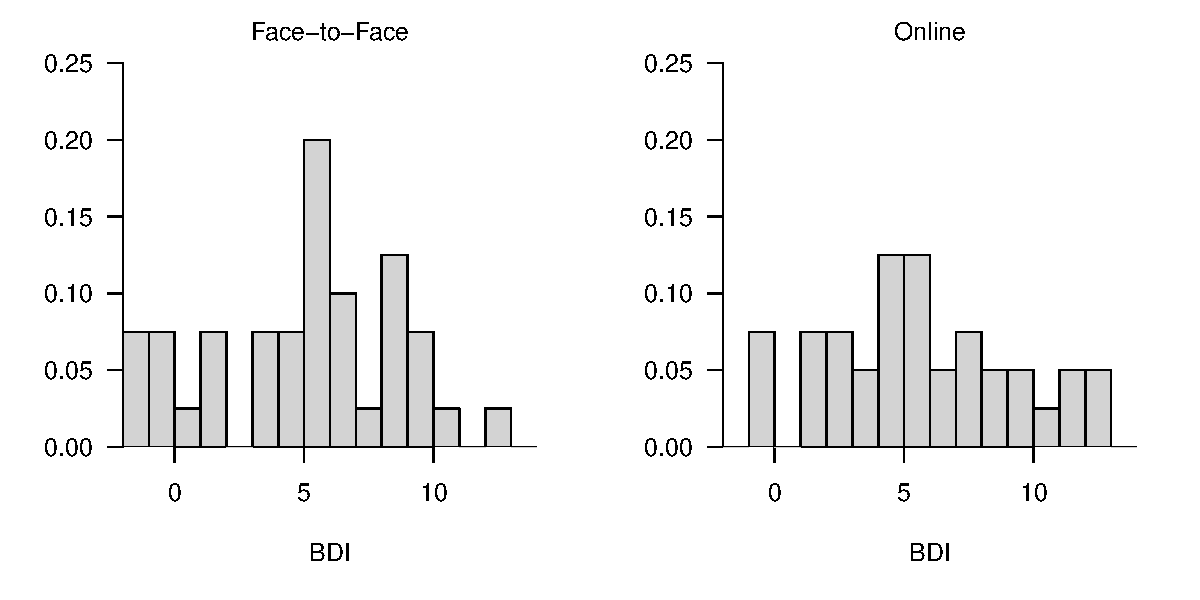
\includegraphics[width=0.95\linewidth]{9_Abbildungen/alm_9_F2F_ONL_histogramme} \end{center}

\setstretch{1}
\footnotesize

\begin{Shaded}
\begin{Highlighting}[]
\CommentTok{\# Ausgabe}
\FunctionTok{print.AsIs}\NormalTok{(S)}
\end{Highlighting}
\end{Shaded}

\begin{verbatim}
>      n Max Min Median Mean  Var  Std
> F2F 40  13  -3      6 5.28 14.8 3.85
> ONL 40  18  -5      6 5.92 25.7 5.07
\end{verbatim}
\end{frame}

\begin{frame}{Zweistichproben-T-Tests}
\protect\hypertarget{zweistichproben-t-tests-2}{}
\large
\setstretch{3}
\vfill

Anwendungsszenario

\textbf{Modellformulierung}

Modellschätzung

Modellevaluation \vfill
\end{frame}

\begin{frame}{Modellformulierung}
\protect\hypertarget{modellformulierung-2}{}
\footnotesize
\begin{definition}[Zweistichproben-T-Test Modell]
\justifying
$y_{ij}$ mit $i = 1,2$ und $j = 1,...,n_i$ seien Zufallsvariablen, die die Datenpunkte
eines Zweistichproben-T-Test Anwendungsszenarios modellieren. Dann hat das
\textit{Zweistichproben-T-Test Modell} die strukturelle Form
\begin{equation}
y_{ij} = \mu_i + \varepsilon_{ij}
\mbox{ mit } \varepsilon_{ij} \sim N(0,\sigma^2)
\mbox{ u.i.v. für } i = 1,2, j = 1,...,n_i \mbox{ mit } \mu_i \in \mathbb{R} \mbox{ und } \sigma^2 > 0,
\end{equation}
die Datenverteilungsform
\begin{equation}
y_{ij} \sim N(\mu_i,\sigma^2)
\mbox{ u.i.v. für } i = 1,2, j = 1,...,n_i \mbox{ mit } \mu_i \in \mathbb{R} \mbox{ und } \sigma^2 > 0,
\end{equation}
und für den Datenvektor $y = (y_{11}, ...,y_{1n_1}, y_{21}, ...,y_{2n_2})^T$ und $n := n_1 + n_2$ die Designmatrixform
\begin{equation}
y = X\beta + \varepsilon \mbox{ mit }
X     := \begin{pmatrix} 1_{n_1} & 0_{n_1} \\ 0_{n_2} & 1_{n_2} \end{pmatrix} \in \mathbb{R}^{n \times 2},
\beta := \begin{pmatrix} \mu_1 \\ \mu_2 \end{pmatrix} \in \mathbb{R}^2,
\varepsilon \sim N(0_n,\sigma^2I_n),
\sigma^2 > 0.
\end{equation}
\end{definition}

Bemerkungen

\begin{itemize}
\tightlist
\item
  \(i\) indiziert die Gruppen, \(j\) indiziert die Daten in jeder
  Gruppe.
\item
  \(n_1\) und \(n_2\) repräsentieren die Gruppengrößen, \(n\)
  repräsentiert die Gesamtanzahl an Datenpunkten.
\item
  Es ist \(p = 2\).
\item
  Die Äquivalenz der drei Modellformen ergibt sich mit den Ergebnissen
  Einheit (5) Modellformulierung.
\end{itemize}
\end{frame}

\begin{frame}[fragile]{Modellformulierung}
\protect\hypertarget{modellformulierung-3}{}
\small

Datensimulation (vgl. Einheit (5) Modellformulierung) \vspace{4mm}

\footnotesize
\setstretch{1.2}

\begin{Shaded}
\begin{Highlighting}[]
\CommentTok{\# Libraries}
\FunctionTok{library}\NormalTok{(MASS)                                }\CommentTok{\# Multivariate Normalverteilung}

\CommentTok{\# Modellformulierung}
\NormalTok{n\_1    }\OtherTok{=} \DecValTok{40}                                  \CommentTok{\# Anzahl von Datenpunkten Gruppe 1}
\NormalTok{n\_2    }\OtherTok{=} \DecValTok{40}                                  \CommentTok{\# Anzahl von Datenpunkten Gruppe 2}
\NormalTok{n      }\OtherTok{=}\NormalTok{ n\_1 }\SpecialCharTok{+}\NormalTok{ n\_2                           }\CommentTok{\# Gesamtanzahl Datenpunkte}
\NormalTok{p      }\OtherTok{=} \DecValTok{2}                                   \CommentTok{\# Anzahl von Betaparameter}
\NormalTok{X      }\OtherTok{=} \FunctionTok{matrix}\NormalTok{(}\FunctionTok{c}\NormalTok{(}\FunctionTok{rep}\NormalTok{(}\DecValTok{1}\NormalTok{,n\_1), }\FunctionTok{rep}\NormalTok{(}\DecValTok{0}\NormalTok{,n\_1),    }\CommentTok{\# Designmatrix}
                  \FunctionTok{rep}\NormalTok{(}\DecValTok{0}\NormalTok{,n\_2), }\FunctionTok{rep}\NormalTok{(}\DecValTok{1}\NormalTok{,n\_2)),}
                  \AttributeTok{nrow  =}\NormalTok{ n)}
\NormalTok{I\_n    }\OtherTok{=} \FunctionTok{diag}\NormalTok{(n)                             }\CommentTok{\# n x n Einheitsmatrix}
\NormalTok{beta   }\OtherTok{=} \FunctionTok{matrix}\NormalTok{(}\FunctionTok{c}\NormalTok{(}\DecValTok{1}\NormalTok{,}\DecValTok{2}\NormalTok{), }\AttributeTok{nrow =}\NormalTok{ p)            }\CommentTok{\# wahrer, aber unbekannter, Betaparameter}
\NormalTok{sigsqr }\OtherTok{=} \DecValTok{14}                                  \CommentTok{\# wahrer, aber unbekannter, Varianzparameter}

\CommentTok{\# Datenrealisierung}
\NormalTok{y      }\OtherTok{=} \FunctionTok{mvrnorm}\NormalTok{(}\DecValTok{1}\NormalTok{, X }\SpecialCharTok{\%*\%}\NormalTok{ beta, sigsqr}\SpecialCharTok{*}\NormalTok{I\_n)  }\CommentTok{\# eine Realisierung eines n{-}dimensionalen ZVs}
\end{Highlighting}
\end{Shaded}
\end{frame}

\begin{frame}{Zweistichproben-T-Tests}
\protect\hypertarget{zweistichproben-t-tests-3}{}
\large
\setstretch{3}
\vfill

Anwendungsszenario

Modellformulierung

\textbf{Modellschätzung}

Modellevaluation \vfill
\end{frame}

\begin{frame}{Modellschätzung}
\protect\hypertarget{modellschuxe4tzung-2}{}
\footnotesize
\begin{theorem}[Parameterschätzung im Zweistichproben-T-Test Modell]
\normalfont
\justifying
Gegeben sei die Designmatrixform des Zweistichproben-T-Test Modells. Dann ergeben
sich für den Betaparameterschätzer
\begin{equation}
\hat{\beta}
=  \begin{pmatrix} \frac{1}{n_1}\sum_{j=1}^{n_1} y_{1j} \\  \frac{1}{n_2}\sum_{j=1}^{n_2} y_{2j} \end{pmatrix}
=: \begin{pmatrix} \bar{y}_1 \\  \bar{y}_2 \end{pmatrix}
\end{equation}
und für den Varianzparameterschätzer
\begin{equation}
\hat{\sigma}^2_{12}
= \frac{\sum_{j=1}^{n_1} (y_{1j} - \bar{y}_1)^2 + \sum_{j=1}^{n_2} (y_{2j} - \bar{y}_2)^2}{n_1+n_2-2}
=: s_{12}^2
\end{equation}
\end{theorem}

Bemerkungen

\begin{itemize}
\tightlist
\item
  \justifying \(\bar{y}_1\) und \(\bar{y}_2\) bezeichnen die
  gruppenspezifischen Stichprobenmittel.
\item
  \(s_{12}^2\) wird als \textit{gepoolte Stichprobenvarianz} bezeichnet.
\item
  Für einen Datensatz \(y = (y_1,y_2)^T \in \mathbb{R}^{n_1 + n_2}\)
  gilt allgemeinen, dass \(s_y^2 \neq s_{12}^2\); die gepoolte
  Stichprobenvarianz und die Stichprobenvarianz eines konkatenierten
  Datensatzes sind im Allgemeinen also nicht identisch. Wir wollen das
  Konzept der gepoolten Stichprobenvarianz hier aber nicht weiter
  vertiefen.
\end{itemize}
\end{frame}

\begin{frame}{Modellschätzung}
\protect\hypertarget{modellschuxe4tzung-3}{}
\footnotesize

\underline{Beweis}

Für \(i = 1,2\) sei \(y_i := (y_{i1},...,y_{in_i})^T\). Dann ergibt sich
für den Betaparameterschätzer \begin{align}
\begin{split}
\hat{\beta}
& = (X^{T}X)^{-1}X^{T}y
\\
& = \left(
\begin{pmatrix} 1_{n_1} & 0_{n_2} \\ 0_{n_1} & 1_{n_2} \end{pmatrix}
\begin{pmatrix} 1_{n_1} & 0_{n_1} \\ 0_{n_2} & 1_{n_2} \end{pmatrix}
\right)^{-1}
\begin{pmatrix} 1_{n_1} & 0_{n_2} \\ 0_{n_1} & 1_{n_2} \end{pmatrix}
\begin{pmatrix} y_1 \\ y_2 \end{pmatrix}
\\
& =
\begin{pmatrix}
n_1     & 0     \\
0       & n_2   \\
\end{pmatrix}^{-1}
\begin{pmatrix}
\sum_{j=1}^{n_1} y_{1j} \\
\sum_{j=1}^{n_2} y_{2j} \\
\end{pmatrix}
\\
& = \begin{pmatrix}
n_1^{-1}    & 0         \\
0           & n_2^{-1}  \\
\end{pmatrix}
\begin{pmatrix}
\sum_{j=1}^{n_1} y_{1j} \\
\sum_{j=1}^{n_2} y_{2j} \\
\end{pmatrix} \\
& =\begin{pmatrix}
\frac{1}{n_1}\sum_{j=1}^{n_1} y_{1j} \\
\frac{1}{n_2}\sum_{j=1}^{n_2} y_{2j} \\
\end{pmatrix}
\\
& =: \begin{pmatrix} \bar{y}_1 \\  \bar{y}_2 \end{pmatrix}.
\end{split}
\end{align}
\end{frame}

\begin{frame}{Modellschätzung}
\protect\hypertarget{modellschuxe4tzung-4}{}
\footnotesize

\underline{Beweis (fortgeführt)}

Gleichsam ergibt sich für Varianzparameterschätzer mit \(n = n_1 + n_2\)
und \(p = 2\) \begin{align}
\begin{split}
\hat{\sigma}^{2}
& =
\frac{(y-X\hat{\beta})^T(y - X\hat{\beta})}{n - p} \\
& =
\frac{1}{n_1+n_2-2}
\left(
\begin{pmatrix} y_1 \\ y_2 \end{pmatrix}
-
\begin{pmatrix} 1_{n_1} & 0_{n_1} \\ 0_{n_2} & 1_{n_2} \end{pmatrix}
\begin{pmatrix}
\bar{y}_{1}\\
\bar{y}_{2}\\
\end{pmatrix}
\right)^{T}
\left(
\begin{pmatrix} y_1 \\ y_2 \end{pmatrix}
-
\begin{pmatrix} 1_{n_1} & 0_{n_1} \\ 0_{n_2} & 1_{n_2} \end{pmatrix}
\begin{pmatrix}
\bar{y}_{1}\\
\bar{y}_{2}\\
\end{pmatrix} \right) \\
& =\frac{1}{n_1+n_2-2}
\begin{pmatrix}
y_{11}-\bar{y}_{1}\\
\vdots \\
y_{1n_1}-\bar{y}_{1}\\
y_{21}-\bar{y}_{2}\\
\vdots \\
y_{2n_2}-\bar{y}_{2}\\
\end{pmatrix}^{T}
\begin{pmatrix}
y_{11}-\bar{y}_{1}\\
\vdots \\
y_{1n_1}-\bar{y}_{1}\\
y_{21}-\bar{y}_{2}\\
\vdots \\
y_{2n_2}-\bar{y}_{2}\\
\end{pmatrix} \\
& = \frac{
    \sum_{j=1}^{n_1} (y_{1j}-\bar{y}_{1})^{2}
   +\sum_{j=1}^{n_2} (y_{2j}-\bar{y}_{2})^{2}
   }{n_1+n_2-2}
\\
& =: s_{12}^2.
\end{split}
\end{align}
\end{frame}

\begin{frame}[fragile]{Modellschätzung}
\protect\hypertarget{modellschuxe4tzung-5}{}
\tiny
\vspace{2mm}
\setstretch{1}

\begin{Shaded}
\begin{Highlighting}[]
\CommentTok{\# Dateneinlesen}
\NormalTok{fname      }\OtherTok{=} \FunctionTok{file.path}\NormalTok{(}\FunctionTok{getwd}\NormalTok{(), }\StringTok{"9\_Daten"}\NormalTok{, }\StringTok{"data\_9\_t\_tests.csv"}\NormalTok{)  }\CommentTok{\# Dateiname}
\NormalTok{D          }\OtherTok{=} \FunctionTok{read.table}\NormalTok{(fname, }\AttributeTok{sep =} \StringTok{","}\NormalTok{, }\AttributeTok{header =} \ConstantTok{TRUE}\NormalTok{)          }\CommentTok{\# Dataframe}
\NormalTok{y\_1        }\OtherTok{=}\NormalTok{ D}\SpecialCharTok{$}\NormalTok{BDI[D}\SpecialCharTok{$}\NormalTok{Condition }\SpecialCharTok{==} \StringTok{"F2F"}\NormalTok{]                          }\CommentTok{\# BDI Differenzwerte in der F2F Gruppe}
\NormalTok{y\_2        }\OtherTok{=}\NormalTok{ D}\SpecialCharTok{$}\NormalTok{BDI[D}\SpecialCharTok{$}\NormalTok{Condition }\SpecialCharTok{==} \StringTok{"ONL"}\NormalTok{]                          }\CommentTok{\# BDI Differenzwerte in der ONL Gruppe}

\CommentTok{\# Modellformulierung}
\NormalTok{n\_1        }\OtherTok{=} \FunctionTok{length}\NormalTok{(y\_1)                                          }\CommentTok{\# Anzahl Datenpunkte Gruppe 1 (F2F)}
\NormalTok{n\_2        }\OtherTok{=} \FunctionTok{length}\NormalTok{(y\_1)                                          }\CommentTok{\# Anzahl Datenpunkte Gruppe 2 (ONL)}
\NormalTok{n          }\OtherTok{=}\NormalTok{ n\_1 }\SpecialCharTok{+}\NormalTok{ n\_2                                            }\CommentTok{\# Gesamtanzahl Datenpunkte}
\NormalTok{y          }\OtherTok{=} \FunctionTok{matrix}\NormalTok{(}\FunctionTok{c}\NormalTok{(y\_1, y\_2), }\AttributeTok{nrow =}\NormalTok{ n)                        }\CommentTok{\# Datenvektor}
\NormalTok{p          }\OtherTok{=} \DecValTok{2}                                                    \CommentTok{\# Anzahl Betaparameter}
\NormalTok{X          }\OtherTok{=} \FunctionTok{matrix}\NormalTok{(}\FunctionTok{c}\NormalTok{(}\FunctionTok{rep}\NormalTok{(}\DecValTok{1}\NormalTok{,n\_1), }\FunctionTok{rep}\NormalTok{(}\DecValTok{0}\NormalTok{,n\_1),                     }\CommentTok{\# Designmatrix}
                      \FunctionTok{rep}\NormalTok{(}\DecValTok{0}\NormalTok{,n\_2), }\FunctionTok{rep}\NormalTok{(}\DecValTok{1}\NormalTok{,n\_2)),}
                      \AttributeTok{nrow  =}\NormalTok{ n)}

\CommentTok{\# Modellschätzung}
\NormalTok{beta\_hat   }\OtherTok{=} \FunctionTok{solve}\NormalTok{(}\FunctionTok{t}\NormalTok{(X) }\SpecialCharTok{\%*\%}\NormalTok{ X) }\SpecialCharTok{\%*\%} \FunctionTok{t}\NormalTok{(X) }\SpecialCharTok{\%*\%}\NormalTok{ y                     }\CommentTok{\# Betaparameterschätzer}
\NormalTok{eps\_hat    }\OtherTok{=}\NormalTok{ y }\SpecialCharTok{{-}}\NormalTok{ X }\SpecialCharTok{\%*\%}\NormalTok{ beta\_hat                                   }\CommentTok{\# Residuenvektor}
\NormalTok{sigsqr\_hat }\OtherTok{=}\NormalTok{ (}\FunctionTok{t}\NormalTok{(eps\_hat) }\SpecialCharTok{\%*\%}\NormalTok{ eps\_hat) }\SpecialCharTok{/}\NormalTok{(n}\SpecialCharTok{{-}}\NormalTok{p)                      }\CommentTok{\# Varianzparameterschätzer}
\NormalTok{s\_sqr\_12   }\OtherTok{=}\NormalTok{ ((n\_1}\DecValTok{{-}1}\NormalTok{)}\SpecialCharTok{*}\FunctionTok{var}\NormalTok{(y\_1) }\SpecialCharTok{+}\NormalTok{ (n\_2}\DecValTok{{-}1}\NormalTok{)}\SpecialCharTok{*}\FunctionTok{var}\NormalTok{(y\_2))}\SpecialCharTok{/}\NormalTok{(n\_1}\SpecialCharTok{+}\NormalTok{n\_2}\DecValTok{{-}2}\NormalTok{)    }\CommentTok{\# gepoolte Stichprobenvarianz}

\CommentTok{\# Ausgabe}
\FunctionTok{cat}\NormalTok{(}\StringTok{"hat\{beta\}          : "}\NormalTok{  , }\FunctionTok{paste}\NormalTok{(beta\_hat),                   }\CommentTok{\# Betaparameterschätzer}
    \StringTok{"}\SpecialCharTok{\textbackslash{}n}\StringTok{bar\{y\}\_1, bar\{y\_2\} : "}\NormalTok{, }\FunctionTok{paste}\NormalTok{( }\FunctionTok{c}\NormalTok{(}\FunctionTok{mean}\NormalTok{(y\_1), }\FunctionTok{mean}\NormalTok{(y\_2))),   }\CommentTok{\# Stichprobenmittel}
    \StringTok{"}\SpecialCharTok{\textbackslash{}n}\StringTok{hat\{sigsqr\}        : "}\NormalTok{, }\FunctionTok{paste}\NormalTok{(sigsqr\_hat),                 }\CommentTok{\# Varianzparameterschätzer}
    \StringTok{"}\SpecialCharTok{\textbackslash{}n}\StringTok{s\_12\^{}2             : "}\NormalTok{, }\FunctionTok{paste}\NormalTok{(s\_sqr\_12),                   }\CommentTok{\# gepoolte Stichprobenvarianz}
    \StringTok{"}\SpecialCharTok{\textbackslash{}n}\StringTok{s\_y\^{}2              : "}\NormalTok{, }\FunctionTok{paste}\NormalTok{(}\FunctionTok{var}\NormalTok{(y)))                     }\CommentTok{\# Stichprobenvarianz des konkatenierten Datensatzes}
\end{Highlighting}
\end{Shaded}

\begin{verbatim}
> hat{beta}          :  5.275 5.925 
> bar{y}_1, bar{y_2} :  5.275 5.925 
> hat{sigsqr}        :  20.2403846153846 
> s_12^2             :  20.2403846153846 
> s_y^2              :  20.0911392405063
\end{verbatim}
\end{frame}

\begin{frame}{Zweistichproben-T-Tests}
\protect\hypertarget{zweistichproben-t-tests-4}{}
\large
\setstretch{3}
\vfill

Anwendungsszenario

Modellformulierung

Modellschätzung

\textbf{Modellevaluation} \vfill
\end{frame}

\begin{frame}{Modellevaluation}
\protect\hypertarget{modellevaluation-24}{}
\small
\setstretch{1.6}

Überblick

\footnotesize

\begin{itemize}
\tightlist
\item
  Wir gruppieren frequentistische Konfidenzintervalle und
  Hypothesentests unter Modellevaluation.
\item
  Wir verzichten an dieser Stelle auf eine Diskussion von
  Konfidenzintervallen
\item
  In der Praxis zielt die Evaluation von Zweistichproben-T-Tests ALM
  Designs meist auf einen Hypothesentest.
\item
  Die Theorie der Zweistichproben-T-Tests ist umfangreich, siehe dazu
  WTFI (14) Zweistichproben-T-Tests.
\item
  Ein gutes Verständnis von WTFI Einheit (12) Hypothesentests wird im
  Folgenden vorausgesetzt.
\end{itemize}

Im Zweistichproben-T-Test ALM Design ergeben sich folgende
Hypothesenszenarien

\begin{itemize}
\tightlist
\item
  \(H_0:\mu_1 - \mu_2 = \mu_0\) und \(H_1: \mu_1 - \mu_2 \neq \mu_0\)
\item
  \(H_0:\mu_1 - \mu_2 \le \mu_0\) und \(H_1: \mu_1 - \mu_2 > \mu_0\)
\item
  \(H_0:\mu_1 - \mu_2 \ge \mu_0\) und \(H_1: \mu_1 - \mu_2 < \mu_0\)
\end{itemize}

Wir betrachten hier nur exemplarisch \(H_0:\mu_1 - \mu_2 = \mu_0\) und
\(H_1: \mu_1 - \mu_2 \neq \mu_0\)

Für \(\mu_0 := 0\) gelten dabei insbesondere

\begin{itemize}
\tightlist
\item
  \(H_0:\mu_1 - \mu_2 = 0 \Leftrightarrow H_0: \mu_1 = \mu_2\)
\item
  \(H_0:\mu_1 - \mu_2 \neq 0 \Leftrightarrow H_0: \mu_1 \neq \mu_2\)
\end{itemize}
\end{frame}

\begin{frame}{Modellevaluation}
\protect\hypertarget{modellevaluation-25}{}
\setstretch{1.8}

\textcolor{darkblue}{Gliederung (vgl. WTFI Einheiten (12) - (14))}

\begin{enumerate}
[(1)]
\item
  Statistisches Modell \checkmark
\item
  Testhypothesen \checkmark
\item
  Teststatistik
\item
  Test
\item
  Analyse der Testgütefunktion
\item
  Testumfangkontrolle
\item
  p-Werte
\item
  Analyse der Powerfunktion
\end{enumerate}
\end{frame}

\begin{frame}{Modellevaluation}
\protect\hypertarget{modellevaluation-26}{}
\noindent (3) Teststatistik

\footnotesize
\begin{theorem}[T-Teststatistik des Zweistichproben-T-Tests]
\justifying
\normalfont
Gegeben sei die Designmatrixform des Zweistichproben-T-Tests. Dann ergibt sich
für die T-Teststatistik mit
\begin{equation}
c := (1,-1)^T \mbox{ und } c^T\beta_0 =: \mu_0,
\end{equation}
dass
\begin{equation}
T = \sqrt{\frac{n_1n_2}{n_1+n_2}}\left(\frac{\bar{y}_1-\bar{y}_2 - \mu_0}{s_{12}}\right)
\end{equation}
und es gilt
\begin{equation}
T \sim t(\delta, n_1 + n_2 - 2) \mbox{ mit } \delta = \sqrt{\frac{n_1n_2}{n_1+n_2}}\left(\frac{\mu_1-\mu_2-\mu_0}{\sigma}\right).
\end{equation}
\end{theorem}

Bemerkungen

\begin{itemize}
\tightlist
\item
  Das Theorem basiert auf dem T-Teststatistik Theorem in Einheit (7)
  Modellevaluation.
\end{itemize}
\end{frame}

\begin{frame}{Modellevaluation}
\protect\hypertarget{modellevaluation-27}{}
\noindent (3) Teststatistik

\footnotesize

\underline{Beweis}

Mit dem T-Teststatistik Theorem in Einheit (7) Modellevaluation gilt
zunächst für die Zähler von \(T\) und \(\delta\), dass \begin{equation}
c^T\hat{\beta} - c^T\beta_0
= \begin{pmatrix} 1         &  - 1       \end{pmatrix}
  \begin{pmatrix} \bar{y}_1 \\ \bar{y}_2 \end{pmatrix}
  - \mu_0
= \bar{y}_1 - \bar{y}_2 - \mu_0
\end{equation} und \begin{equation}
c^T\beta - c^T\beta_0
= \begin{pmatrix} 1     &  - 1    \end{pmatrix}
  \begin{pmatrix} \mu_1 \\ \mu_2  \end{pmatrix}
  - \mu_0
= \mu_1 - \mu_2 - \mu_0,
\end{equation} respektive. Weiterhin gilt für die Nenner von \(T\) und
\(\delta\), dass \begin{equation}
c^T(X^TX)^{-1}c =
\begin{pmatrix*}[r] 1        & - 1 \end{pmatrix*}
\begin{pmatrix} n_1^{-1} & 0        \\
                0        & n_2^{-1}
\end{pmatrix}
\begin{pmatrix*}[r] 1       \\ - 1 \end{pmatrix*}
=
\begin{pmatrix*}[r] n_1^{-1} &  - n_2^{-1} \end{pmatrix*}
\begin{pmatrix*}[r] 1        \\ - 1 \end{pmatrix*}
= \frac{1}{n_1} + \frac{1}{n_2}
\end{equation} Außerdem gilt \begin{equation}
  \left(\frac{1}{n_1} + \frac{1}{n_2}\right)^{-\frac{1}{2}}
= \left(\frac{n_2}{n_1n_2} + \frac{n_1}{n_1n_2}\right)^{-\frac{1}{2}}
= \left(\frac{n_1 + n_2}{n_1n_2}\right)^{-\frac{1}{2}}
= \left(\frac{n_1n_2}{n_1+n_2}\right)^{\frac{1}{2}}
\end{equation} Zusammengenommen folgt direkt, dass \begin{equation}
T = \sqrt{\frac{n_1n_2}{n_1+n_2}}\left(\frac{\bar{y}_1-\bar{y}_2 - \mu_0}{s_{12}}\right)
\mbox{ und }
\delta = \sqrt{\frac{n_1n_2}{n_1+n_2}}\left(\frac{\mu_1-\mu_2-\mu_0}{\sigma}\right).
\end{equation}
\end{frame}

\begin{frame}{Modellevaluation}
\protect\hypertarget{modellevaluation-28}{}
\noindent (4) Test

\footnotesize
\begin{definition}[Zweiseitiger Zweistichproben-T-Test]
\justifying
Gegeben sei das Zweistichproben-T-Test Modell. Für ein $\mu_0 \in \mathbb{R}$ seien
die einfache Nullhypothese und die zusammgensetzte Alternativhypothese gegeben durch
\begin{equation}
H_0 : \mu_1 - \mu_2 = \mu_0
\Leftrightarrow
\Theta_0 := \{(\mu_1,\mu_2) \in \mathbb{R}^2|\mu_1 - \mu_2 = \mu_0\}
\end{equation}
und
\begin{equation}
H_1 : \mu_1 - \mu_2 \neq \mu_0
\Leftrightarrow
\Theta_1 := \{(\mu_1,\mu_2) \in \mathbb{R}^2|\mu_1 - \mu_2 \neq \mu_0\},
\end{equation}
respektive. Weiterhin sei die T-Teststatistik definiert durch
\begin{equation}
T := \sqrt{\frac{n_1n_2}{n_1+n_2}}\left(\frac{\bar{y}_1-\bar{y}_2}{s_{12}}\right)
\end{equation}
Dann ist der zweiseitige \textit{Zweistichproben-T-Teststatistik} definiert als
der kritischen Wert-basierte Test
\begin{equation}
\phi(y) := 1_{\{|T| \ge k\}}.
\end{equation}
\end{definition}

Bemerkungen

\begin{itemize}
\tightlist
\item
  Ausführlicher handelt es sich um den \emph{zweiseitigen
  Zweistichproben-T-Test mit ungerichteter Hypothese}.
\end{itemize}
\end{frame}

\begin{frame}{Modellevaluation}
\protect\hypertarget{modellevaluation-29}{}
\setstretch{1.1}

\noindent (5) Analyse der Testgütefunktion

\footnotesize
\begin{theorem}[Testgütefunktion]
\justifying
\normalfont
Es sei $\phi$ der im obigen Modell formulierte Zweistichproben-T-Test. Dann ist
die Testgütefunktion von $\phi$ gegeben durch
\begin{multline}
q_{\phi} : \mathbb{R}^2 \to [0,1],
(\mu_1, \mu_2) \mapsto q_{\phi}(\mu_1, \mu_2)
\\ := 1 - \psi(k;d_{\mu_1,\mu_2},n_1+n_2-2) + \psi(-k;d_{\mu_1,\mu_2},n_1+n_2-2)
\end{multline}
wobei $\psi(\cdot; d_{\mu_1,\mu_2}, n_1+n_2-2)$  die KVF der nichtzentralen
$t$-Verteilung mit Nichtzentralitätsparameter
\begin{equation}
d_{\mu_1,\mu_2} := \sqrt{\frac{n_1n_2}{n_1+n_2}}\frac{\mu_1-\mu_2}{\sigma}
\end{equation}
und Freiheitsgradparameter $n_1+n_2-2$ bezeichnet.
\end{theorem}

Bemerkungen

\begin{itemize}
\tightlist
\item
  \(q_{\phi}\) ist eine bivariate reellwertige Funktion.
\item
  \(q_{\phi}\) kann alternativ als univariate reellwertige Funktion von
  \(\Delta := \mu_1 - \mu_2\) konzipiert werden.
\item
  Im Vergleich zum Einstichprobenszenario gelten \begin{equation}
  n \hookrightarrow n_1+n_2-2,\quad\quad
  \sqrt{n} \hookrightarrow \sqrt{\frac{n_1n_2}{n_1 + n_2}},\quad\quad
  \mu - \mu_0  \hookrightarrow \mu_1 - \mu_2
  \end{equation}
\item
  Für einen Beweisansatz, siehe DeGroot and Schervish (2012) Seite 591.
\end{itemize}
\end{frame}

\begin{frame}{Modellevaluation}
\protect\hypertarget{modellevaluation-30}{}
\setstretch{1.1}

\noindent (5) Analyse der Testgütefunktion \vfill

\center Testgütefunktion \(q_\phi\) für
\(\sigma^2 = 9, n_1 = 12, n_2 = 12\). \vspace{2mm} \begin{equation*}
q_{\phi}(\mu) = \mathbb{P}_\mu(\phi = 1)
\end{equation*} \vspace{1mm}

\begin{center}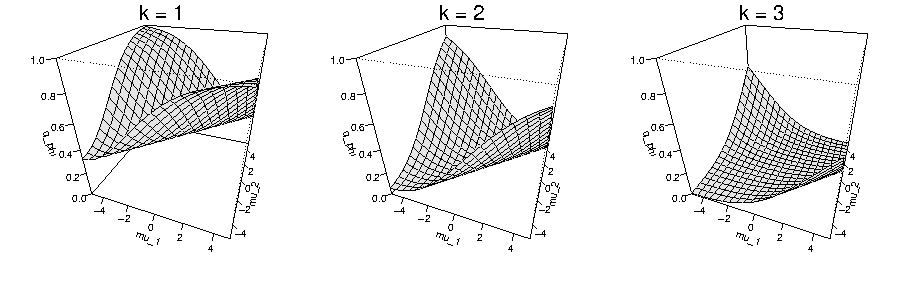
\includegraphics[width=1\linewidth]{9_Abbildungen/alm_9_t_test_q_phi_zweistichproben} \end{center}
\vfill
\end{frame}

\begin{frame}{\small Modellevaluation}
\protect\hypertarget{modellevaluation-31}{}
\noindent (6) Testumfangkontrolle \vfill \small

\begin{theorem}[Testumfangkontrolle]
\justifying
\normalfont
$\phi$ sei der im obigen Testszenario definierte Test. Dann ist $\phi$ ein
Level-$\alpha_0$-Test mit Testumfang $\alpha_0$, wenn der kritische Wert
definiert ist durch
\begin{equation}
k_{\alpha_0} := \psi^{-1}\left(1 - \frac{\alpha_0}{2}; n_1 + n_2 - 2 \right),
\end{equation}
wobei $\psi^{-1}(\cdot; n_1+n_2-2)$ die inverse KVF der $t$-Verteilung mit
$n_1+n_2-2$ Freiheitsgraden ist.
\end{theorem}

Bemerkungen

\begin{itemize}
\tightlist
\item
  Das Resultat folgt in Analogie zum Einstichproben-T-Test.
\item
  Im Vergleich zum Einstichproben-T-Testfall gilt lediglich
  \begin{equation}
  n - 1 \hookrightarrow n_1 + n_2 - 2.
  \end{equation} \vfill
\end{itemize}
\end{frame}

\begin{frame}{Modellevaluation}
\protect\hypertarget{modellevaluation-32}{}
\noindent (6) Testumfangkontrolle

\small

Praktisches Vorgehen \footnotesize

\begin{itemize}
\itemsep1mm
\justifying

\item Man nimmt an, dass die Daten zweier Gruppen $\upsilon_{11},...,\upsilon_{1n_1}$
und $\upsilon_{21},...,\upsilon_{2n_2}$ Realisationen von
$y_{1j} \sim N(\mu_1,\sigma^2) \mbox{ u.i.v.  für } j = 1,...,n_1$ und
$y_{2j} \sim N(\mu_2,\sigma^2) \mbox{ u.i.v.  für } j = 1,...,n_2$
mit unbekannten Parametern $\mu_1,\mu_2,\sigma^2$ sind.

\item Man möchte entscheiden, ob eher $H_0 : \mu_1 - \mu_2 = \mu_0$ oder
$H_1: \mu_1 - \mu_2 \neq \mu_0$ zutrifft.

\item Man wählt ein Signifikanzniveau $\alpha_0$ und bestimmt den zugehörigen
Freiheitsgradparameter-abhängigen kritischen Wert $k_{\alpha_0}$. Zum Beispiel
gilt bei Wahl von $\alpha_0  := 0.05$ und $n_1=12, n_2 = 12$, also
Freiheitsgradparameter 12+12-2 = 22, dass $k_{0.05}=\psi^{-1}(1-0.05/2; 22)
\approx 2.07$ ist.

\item Anhand von $n_1,n_2,\bar{\upsilon}_1,\bar{\upsilon}_2$ und der gepoolten
Stichprobenstandardabweichung $s_{12}$ berechnet man die Realisierung der
Zweistichproben-T-Teststatistik
\begin{equation}
t := \sqrt{\frac{n_1n_2}{n_1+n_2}}\left(\frac{\bar{\upsilon}_1-\bar{\upsilon}_2}{s_{12}}\right)
\end{equation}

\item Wenn $t$ größer-gleich $k_{\alpha_0}$ ist oder wenn $t$ kleiner-
gleich $-k_{\alpha_0}$ ist, lehnt man die Nullhypothese ab, andernfalls lehnt
man sie nicht ab.

\item Die oben entwickelte Theorie des Zweistichproben-T-Tests garantiert dann,
dass man in höchstens $\alpha_0 \cdot 100$ von $100$ Fällen die Nullhypothese
fälschlicherweise ablehnt.
\end{itemize}
\end{frame}

\begin{frame}{Modellevaluation}
\protect\hypertarget{modellevaluation-33}{}
\begin{enumerate}
[(1)]
\setcounter{enumi}{6}
\tightlist
\item
  p-Werte
\end{enumerate}

\small

Bestimmung des p-Wertes \vspace{2mm}

\footnotesize

\begin{itemize}
\item
  \itemsep2mm \justifying \small Per Definition ist der p-Wert das
  kleinste Signifikanzlevel \(\alpha_0\), bei welchem man die
  Nullhypothese basierend auf einem vorliegendem Wert der Teststatistik
  ablehnen würde.
\item
  Bei \(T = t\) würde \(H_0\) für jedes \(\alpha_0\) mit
  \(|t|\ge\psi^{-1}(1-\alpha_0/2; n_1 + n_2-2)\) abgelehnt werden. Für
  diese \(\alpha_0\) gilt, wie bereits mehrfach gezeigt,
  \begin{equation}
  \alpha_0 \ge 2 \mathbb{P}(T \ge |t|).
  \end{equation}
\item
  Das kleinste \(\alpha_0 \in [0,1]\) mit
  \(\alpha_0 \ge 2 \mathbb{P}(T \ge |t|)\) ist dann
  \(\alpha_0 = 2 \mathbb{P}(T \ge |t|)\), also folgt \begin{equation}
  \mbox{p-Wert} =  2 \mathbb{P}(T \ge |t|) = 2(1 - \psi(|t|;n_1 + n_2 - 2)).
  \end{equation}
\item
  Im Vergleich zum Einstichprobenfall gilt lediglich
  \(n \hookrightarrow n_1 + n_2 -2\).
\end{itemize}
\end{frame}

\begin{frame}[fragile]{Modellevaluation}
\protect\hypertarget{modellevaluation-34}{}
\vspace{1mm}
\small

\textcolor{darkblue}{Anwendungszenario} \vspace{1mm} \setstretch{.8}
\tiny

\begin{Shaded}
\begin{Highlighting}[]
\CommentTok{\# Dateneinlesen}
\NormalTok{fname      }\OtherTok{=} \FunctionTok{file.path}\NormalTok{(}\FunctionTok{getwd}\NormalTok{(), }\StringTok{"9\_Daten"}\NormalTok{, }\StringTok{"data\_9\_t\_tests.csv"}\NormalTok{)  }\CommentTok{\# Dateiname}
\NormalTok{D          }\OtherTok{=} \FunctionTok{read.table}\NormalTok{(fname, }\AttributeTok{sep =} \StringTok{","}\NormalTok{, }\AttributeTok{header =} \ConstantTok{TRUE}\NormalTok{)          }\CommentTok{\# Dataframe}
\NormalTok{y\_1        }\OtherTok{=}\NormalTok{ D}\SpecialCharTok{$}\NormalTok{BDI[D}\SpecialCharTok{$}\NormalTok{Condition }\SpecialCharTok{==} \StringTok{"F2F"}\NormalTok{]                          }\CommentTok{\# BDI Differenzwerte in der F2F Gruppe}
\NormalTok{y\_2        }\OtherTok{=}\NormalTok{ D}\SpecialCharTok{$}\NormalTok{BDI[D}\SpecialCharTok{$}\NormalTok{Condition }\SpecialCharTok{==} \StringTok{"ONL"}\NormalTok{]                          }\CommentTok{\# BDI Differenzwerte in der ONL Gruppe}

\CommentTok{\# Modellformulierung}
\NormalTok{n\_1        }\OtherTok{=} \FunctionTok{length}\NormalTok{(y\_1)                                          }\CommentTok{\# Anzahl Datenpunkte Gruppe 1 (F2F)}
\NormalTok{n\_2        }\OtherTok{=} \FunctionTok{length}\NormalTok{(y\_1)                                          }\CommentTok{\# Anzahl Datenpunkte Gruppe 2 (ONL)}
\NormalTok{n          }\OtherTok{=}\NormalTok{ n\_1 }\SpecialCharTok{+}\NormalTok{ n\_2                                            }\CommentTok{\# Gesamtanzahl Datenpunkte}
\NormalTok{y          }\OtherTok{=} \FunctionTok{matrix}\NormalTok{(}\FunctionTok{c}\NormalTok{(y\_1, y\_2), }\AttributeTok{nrow =}\NormalTok{ n)                        }\CommentTok{\# Datenvektor}
\NormalTok{p          }\OtherTok{=} \DecValTok{2}                                                    \CommentTok{\# Anzahl Betaparameter}
\NormalTok{X          }\OtherTok{=} \FunctionTok{matrix}\NormalTok{(}\FunctionTok{c}\NormalTok{(}\FunctionTok{rep}\NormalTok{(}\DecValTok{1}\NormalTok{,n\_1), }\FunctionTok{rep}\NormalTok{(}\DecValTok{0}\NormalTok{,n\_1),                     }\CommentTok{\# Designmatrix}
                      \FunctionTok{rep}\NormalTok{(}\DecValTok{0}\NormalTok{,n\_2), }\FunctionTok{rep}\NormalTok{(}\DecValTok{1}\NormalTok{,n\_2)),}
                      \AttributeTok{nrow  =}\NormalTok{ n)}

\CommentTok{\# Modellschätzung}
\NormalTok{beta\_hat   }\OtherTok{=} \FunctionTok{solve}\NormalTok{(}\FunctionTok{t}\NormalTok{(X) }\SpecialCharTok{\%*\%}\NormalTok{ X) }\SpecialCharTok{\%*\%} \FunctionTok{t}\NormalTok{(X) }\SpecialCharTok{\%*\%}\NormalTok{ y                     }\CommentTok{\# Betaparameterschätzer}
\NormalTok{eps\_hat    }\OtherTok{=}\NormalTok{ y }\SpecialCharTok{{-}}\NormalTok{ X }\SpecialCharTok{\%*\%}\NormalTok{ beta\_hat                                   }\CommentTok{\# Residuenvektor}
\NormalTok{sigsqr\_hat }\OtherTok{=}\NormalTok{ (}\FunctionTok{t}\NormalTok{(eps\_hat) }\SpecialCharTok{\%*\%}\NormalTok{ eps\_hat) }\SpecialCharTok{/}\NormalTok{(n}\SpecialCharTok{{-}}\NormalTok{p)                      }\CommentTok{\# Varianzparameterschätzer}

\CommentTok{\# Modellevaluation}
\NormalTok{c          }\OtherTok{=} \FunctionTok{matrix}\NormalTok{(}\FunctionTok{c}\NormalTok{(}\DecValTok{1}\NormalTok{,}\SpecialCharTok{{-}}\DecValTok{1}\NormalTok{), }\AttributeTok{nrow =} \DecValTok{2}\NormalTok{)                            }\CommentTok{\# Kontrastgewichtsvektor}
\NormalTok{mu\_0       }\OtherTok{=} \DecValTok{0}                                                    \CommentTok{\# Nullhypothese H\_0}
\NormalTok{alpha\_0    }\OtherTok{=} \FloatTok{0.05}                                                 \CommentTok{\# Signifikanzniveau}
\NormalTok{k\_alpha\_0  }\OtherTok{=} \FunctionTok{qt}\NormalTok{(}\DecValTok{1} \SpecialCharTok{{-}}\NormalTok{ (alpha\_0}\SpecialCharTok{/}\DecValTok{2}\NormalTok{), n}\DecValTok{{-}1}\NormalTok{)                             }\CommentTok{\# kritischer Wert}
\NormalTok{t\_num      }\OtherTok{=} \FunctionTok{t}\NormalTok{(c) }\SpecialCharTok{\%*\%}\NormalTok{ beta\_hat }\SpecialCharTok{{-}}\NormalTok{ mu\_0                             }\CommentTok{\# T{-}Teststatistik Zähler}
\NormalTok{t\_den      }\OtherTok{=} \FunctionTok{sqrt}\NormalTok{(sigsqr\_hat}\SpecialCharTok{*}\FunctionTok{t}\NormalTok{(c) }\SpecialCharTok{\%*\%} \FunctionTok{solve}\NormalTok{(}\FunctionTok{t}\NormalTok{(X) }\SpecialCharTok{\%*\%}\NormalTok{ X)}\SpecialCharTok{\%*\%}\NormalTok{c)      }\CommentTok{\# T{-}Teststatistik Nenner}
\NormalTok{t          }\OtherTok{=}\NormalTok{ t\_num}\SpecialCharTok{/}\NormalTok{t\_den                                          }\CommentTok{\# T{-}Teststatistik}
\ControlFlowTok{if}\NormalTok{(}\FunctionTok{abs}\NormalTok{(t) }\SpecialCharTok{\textgreater{}=}\NormalTok{ k\_alpha\_0)\{                                          }\CommentTok{\# Test 1\_\{|T(X) \textgreater{}= k\_alpha\_0|\}}
\NormalTok{    phi }\OtherTok{=} \DecValTok{1}                                                       \CommentTok{\# Ablehnen von H\_0}
\NormalTok{\} }\ControlFlowTok{else}\NormalTok{ \{}
\NormalTok{    phi }\OtherTok{=} \DecValTok{0}                                                       \CommentTok{\# Nicht Ablehnen von H\_0}
\NormalTok{\}}
\NormalTok{pval      }\OtherTok{=} \DecValTok{2}\SpecialCharTok{*}\NormalTok{(}\DecValTok{1}\SpecialCharTok{{-}}\FunctionTok{pt}\NormalTok{(}\FunctionTok{abs}\NormalTok{(t), n\_1}\SpecialCharTok{+}\NormalTok{n\_2}\DecValTok{{-}2}\NormalTok{))                           }\CommentTok{\# p{-}Wert}
\end{Highlighting}
\end{Shaded}

\vspace{-1mm}

\begin{verbatim}
> fg        =  78 
> t         =  -0.646 
> alpha_0   =  0.05 
> k_alpha_0 =  1.99 
> phi       =  0 
> p-Wert    =  0.52
\end{verbatim}
\end{frame}

\begin{frame}[fragile]{Modellevaluation}
\protect\hypertarget{modellevaluation-35}{}
\vspace{1mm}
\small

\textcolor{darkblue}{Anwendungszenario} \vspace{1mm} \setstretch{1}
\tiny

\begin{Shaded}
\begin{Highlighting}[]
\CommentTok{\# Automatischer Zweistichproben{-}T{-}Test}
\NormalTok{varphi    }\OtherTok{=} \FunctionTok{t.test}\NormalTok{(                           }\CommentTok{\# ?t.test für Details}
\NormalTok{            y\_1,                              }\CommentTok{\# Datensatz y\_1}
\NormalTok{            y\_2,                              }\CommentTok{\# Datensatz y\_2}
            \AttributeTok{var.equal   =} \ConstantTok{TRUE}\NormalTok{,               }\CommentTok{\# \textbackslash{}sigma\_1\^{}2 = \textbackslash{}sigma\_2\^{}2}
            \AttributeTok{alternative =} \FunctionTok{c}\NormalTok{(}\StringTok{"two.sided"}\NormalTok{),     }\CommentTok{\# H\_1: \textbackslash{}mu\_1 \textbackslash{}neq \textbackslash{}mu\_2}
            \AttributeTok{conf.level  =} \DecValTok{1}\SpecialCharTok{{-}}\NormalTok{alpha\_0)          }\CommentTok{\# \textbackslash{}delta = 1 {-} \textbackslash{}alpha\_0 (sic!)}

\CommentTok{\# Ausgabe}
\FunctionTok{print}\NormalTok{(varphi)}
\end{Highlighting}
\end{Shaded}

\begin{verbatim}
> 
>   Two Sample t-test
> 
> data:  y_1 and y_2
> t = -0.6, df = 78, p-value = 0.5
> alternative hypothesis: true difference in means is not equal to 0
> 95 percent confidence interval:
>  -2.65  1.35
> sample estimates:
> mean of x mean of y 
>      5.28      5.92
\end{verbatim}

\begin{Shaded}
\begin{Highlighting}[]
\CommentTok{\# Genauere Ausgabe t}
\FunctionTok{paste}\NormalTok{(varphi[}\DecValTok{1}\NormalTok{])}
\end{Highlighting}
\end{Shaded}

\begin{verbatim}
> [1] "c(t = -0.646128613569434)"
\end{verbatim}

\begin{Shaded}
\begin{Highlighting}[]
\CommentTok{\# Genauere Ausgabe p}
\FunctionTok{paste}\NormalTok{(varphi[}\DecValTok{3}\NormalTok{])}
\end{Highlighting}
\end{Shaded}

\begin{verbatim}
> [1] "0.520092604281206"
\end{verbatim}
\end{frame}

\begin{frame}{Modellevaluation}
\protect\hypertarget{modellevaluation-36}{}
\noindent (8) Analyse der Powerfunktion

\small

Wir betrachten die Testgütefunktion \begin{multline}
q_{\phi} : \mathbb{R}^2 \to [0,1],
(\mu_1, \mu_2) \mapsto q_{\phi}(\mu_1, \mu_2)
\\ := 1 - \psi(k;d_{\mu_1,\mu_2},n_1+n_2-2) + \psi(-k;d_{\mu_1,\mu_2},n_1+n_2-2)
\end{multline} als Funktion des Nichtzentralitätsparameters und der
Summe der Stichprobenumfänge \(n := n_1 + n_2\) bei kontrolliertem
Testumfang, also für \(k_{\alpha_0} := \psi^{-1}(1-\alpha_0/2;n-2)\) mit
festem \(\alpha_0\).

Es ergibt sich die multivariate reellwertige Funktion \begin{multline}
\pi : \mathbb{R} \times \mathbb{N}^2 \to [0,1],
(d,n) \mapsto
\\ \pi(d,n) := 1-\psi(k_{\alpha_0};d,n-2)+\psi(-k_{\alpha_0}; d,n-2)
\end{multline} Bei festgelegten \(\alpha_0\) hängt die Powerfunktion des
zweiseitigen T-Tests mit einfacher Nullhypothese also vom unbekannten
Wert \(d\) und von der Summe der Stichprobengrößen \(n\) ab. De-facto
handelt es sich also um die gleiche Powerfunktion wie beim zweiseitigen
Einstichproben-T-Test mit dem einzigen Unterschied, dass für den
Freiheitsgradparameter \(n-2\) anstelle von \(n-1\) gilt. Wir verzichten
auf eine erneute Visualisierung. \vfill
\end{frame}

\begin{frame}{Modellevaluation}
\protect\hypertarget{modellevaluation-37}{}
\noindent (8) Analyse der Powerfunktion

\setstretch{1.2}
\small

Praktisches Vorgehen

Mit größerem \(n = n_1 + n_2\) steigt die Powerfunktion des Tests an

\begin{itemize}
\item
  Ein großer Stichprobenumfang ist besser als ein kleiner
  Stichprobenumfang.
\item
  Kosten für die Erhöhung des Stichprobenumfangs werden aber nicht
  berücksichtigt.
\item
  \justifying Ungleichgewichte zwischen \(n_1\) und \(n_2\) werden durch
  die Tatsache ausglichen, dass Datenpunkte einer Stichproben auch zur
  Varianzschätzung in der anderen Stichprobe beitragen, da eine
  identische Varianz vorausgesetzt wurde.
\end{itemize}

\vspace{1mm}

Die Powerfunktion hängt vom wahren, aber unbekannten, Parameterwert
\(d = \sqrt{n}(\mu_1 - \mu_0)/\sigma\) ab.

\(\Rightarrow\) Wenn man \(d\) schon kennen würde, würde man den Test
nicht durchführen.

\vspace{1mm}

Generell wird folgendes Vorgehen favorisiert

\begin{itemize}
\item
  Man legt das Signifikanzniveau \(\alpha_0\) fest und evaluiert die
  Powerfunktion.
\item
  Man wählt einen Mindestparameterwert \(d^*\), den man mit
  \(\pi(d,n) = b\) detektieren möchte.
\item
  Ein konventioneller Wert ist \(b= 0.8\).
\item
  Man liest die für \(\pi(d = d^*,n) = b\) nötige Stichprobengröße \(n\)
  ab.
\end{itemize}
\end{frame}

\begin{frame}{Modellevaluation}
\protect\hypertarget{modellevaluation-38}{}
\noindent (8) Analyse der Powerfunktion

\small

Praktisches Vorgehen \vspace{5mm}

\begin{center}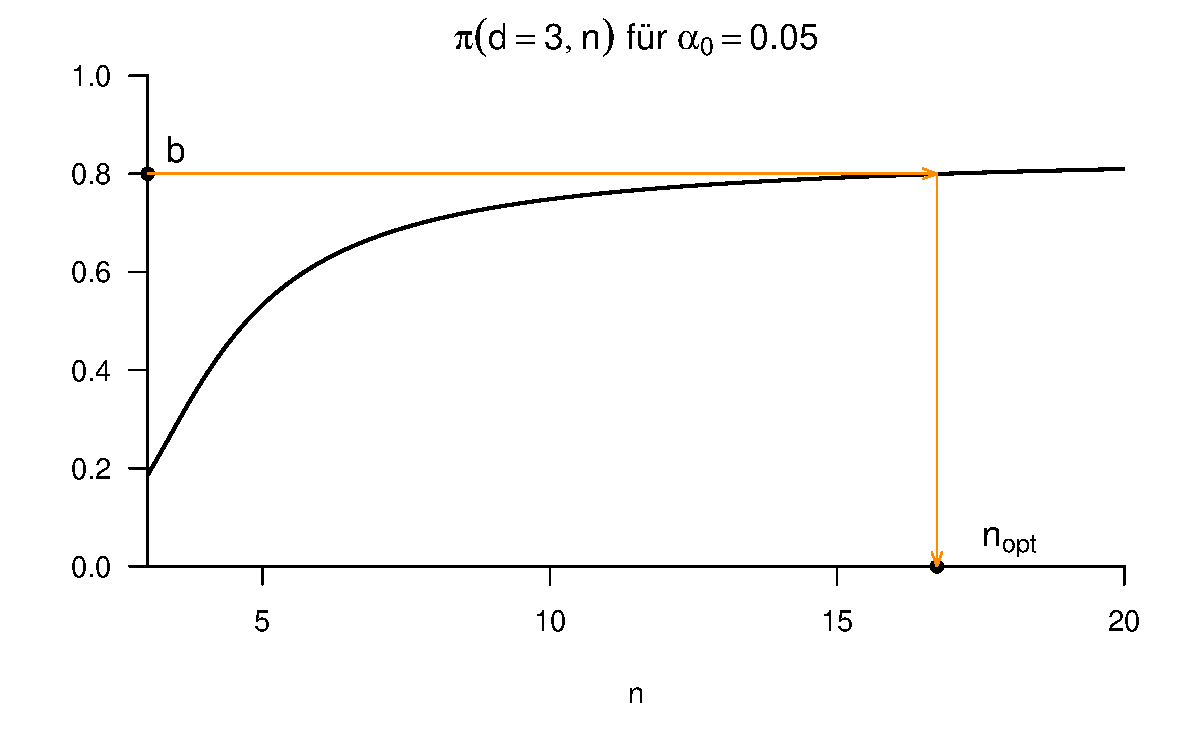
\includegraphics[width=0.8\linewidth]{9_Abbildungen/alm_9_t_test_zweistichproben_umfang} \end{center}
\end{frame}

\begin{frame}{Selbstkontrollfragen}
\protect\hypertarget{selbstkontrollfragen}{}
\footnotesize
\setstretch{1.2}
\begin{enumerate}
\justifying
\itemsep0mm
\item Erläutern Sie die Extremszenarien im Kontinuum von ALM Designs.
\item Erläutern Sie die Begriffe der faktoriellen und parametrischen ALM Designs.
\item Nennen Sie Beispiele für faktorielle, parametrische, und faktoriell-parametrische ALM Designs.
\item Erläutern Sie das Anwendungsszenario eines Einstichproben-T-Tests.
\item Erläutern Sie mögliche Hypothesenszenarien eines Einstichproben-T-Tests.
\item Geben Sie die Definition des Einstichproben-T-Test Modells wieder.
\item Geben Sie das Theorem zur Parameterschätzung im Einstichproben-T-Test Modell wieder.
\item Geben Sie das Theorem zur T-Teststatistik des Einstichproben-T-Tests wieder.
\item Geben Sie die Definition des zweiseitigen Einstichproben-T-Tests (mit ungerichteter Hypothese) wieder.
\item Skizzieren Sie die Testgütefunktion des zweiseitigen Einstichproben-T-Tests.
\item Geben Sie das Theorem zur Testumfangkontrolle im zweiseitigen Level-$\alpha_0$-Einstichproben-T-Test wieder.
\item Erläutern Sie das praktische Vorgehen bei Durchführung eines zweiseitigen Level-$\alpha_0$-Einstichproben-T-Tests.
\item Geben Sie die Definition des p-Wertes Werts für einen zweiseitigen Einstichproben-T-Test wieder.
\item Von welchen Werten hängt die Powerfunktion eines zweiseitigen Einstichproben-T-Tests ab?
\item Skizzieren Sie die Powerfunktion des zweiseitigen Einstichproben-T-Tests bei fester Stichprobengröße.
\item Skizzieren Sie die Powerfunktion des zweiseitigen Einstichproben-T-Tests bei festem Nichtzentralitätsparameter.
\item Betrachten Sie die PostBDI-PreBDI Differenzwertdaten der Waitlist Control Bedingung im Beispieldatensatz. Erstellen
Sie ein Histogramm dieser Daten und evaluieren Sie Ihnen bekannte deskriptive Statistiken zu diesen Daten. Führen Sie
einen zweiseitigen Einstichproben-T-Test mit Nullhypothesenparameter $\mu_0 = 0$ durch. Dokumentieren Sie Ihre Ergebnisse.
Was folgern Sie aus den sich ergebenen Resultaten?
\end{enumerate}
\end{frame}

\begin{frame}{Selbstkontrollfragen}
\protect\hypertarget{selbstkontrollfragen-1}{}
\footnotesize
\setstretch{1.2}
\begin{enumerate}
\justifying
\itemsep0mm
\setcounter{enumi}{17}
\item Erläutern Sie das Anwendungsszenario eines Zweistichproben-T-Tests.
\item Geben Sie die Definition des Zweistichproben-T-Test Modells wieder.
\item Geben Sie das Theorem zur Parameterschätzung im Zweistichproben-T-Test Modell wieder.
\item Geben Sie das Theorem zur T-Teststatistik des Zweistichproben-T-Tests wieder.
\item Erläutern Sie mögliche Hypothesenszenarien eines Zweistichproben-T-Tests.
\item Geben Sie die Definition des zweiseitigen Zweistichproben-T-Tests (mit ungerichteter Hypothese) wieder.
\item Skizzieren Sie die Testgütefunktion des zweiseitigen Zweistichproben-T-Tests.
\item Geben Sie das Theorem zur Testumfangkontrolle im zweiseitigen Level-$\alpha_0$-Zweistichproben-T-Test wieder.
\item Erläutern Sie das praktische Vorgehen bei Durchführung eines zweiseitigen Level-$\alpha_0$-Zweistichproben-T-Tests.
\item Geben Sie die Definition des p-Wertes Werts für einen zweiseitigen Zweistichproben-T-Test wieder.
\item Von welchen Werten hängt die Powerfunktion eines zweiseitigen Zweistichproben-T-Tests ab?
\item Skizzieren Sie die Powerfunktion des zweiseitigen Zweistichproben-T-Tests bei fester Stichprobengröße.
\item Skizzieren Sie die Powerfunktion des zweiseitigen Zweistichproben-T-Tests bei festem Nichtzentralitätsparameter.
\item Betrachten Sie die Daten zum Alter der Patient:innen in der Face-to-Face und Online Therapie Bedingung im Beispieldatensatz. 
Erstellen gruppenspezifische Histogramme dieser Daten und evaluieren Sie gruppenspezifische deskriptive Statistiken zu diesen Daten. Führen Sie
einen zweiseitigen Zweistichproben-T-Test mit Nullhypothesenparameter $\mu_0 = 0$ durch. Dokumentieren Sie Ihre Ergebnisse.
Was folgern Sie aus den sich ergebenen Resultaten?
\end{enumerate}
\end{frame}

\begin{frame}{References}
\protect\hypertarget{references}{}
\footnotesize

\hypertarget{refs}{}
\begin{CSLReferences}{1}{0}
\leavevmode\hypertarget{ref-degroot_2012}{}%
DeGroot, Morris H., and Mark J. Schervish. 2012. \emph{Probability and
Statistics}. 4th ed. {Boston}: {Addison-Wesley}.

\end{CSLReferences}
\end{frame}

\end{document}
